\chapter{Results of dynamic analysis}
\label{chap4}

\section{Modal analysis}
\label{sec:modal analysis}
Modal masses, natural frequencies and mode shapes are the output of modal analysis, they reflect the dynamic characteristics of the floors. It is meaningful to observe how the input geometric parameters $l, l/d, t_v/t_r$ influence the modal parameters.

To measure the relation between input and output, IOC (input/output correlations) value is introduced. IOC is defined as follows:
\begin{equation}
    IOC_i=\rho_{X_i,Y}=\frac{Cov[X_i,Y]}{\sigma_{X_i}\sigma_Y}
\end{equation}
\noindent
where $\rho$ is Pearson's linear correlation coefficient, $X_i$ is one of the input data sets and $Y$ the output data set, $Cov$ stands for covariance and $\sigma$ the standard deviation. If $|\rho_{X_i,Y}|\approx0$, $X_i$ has no importance. Positive/negative values indicate the increasing/decreasing trend of the mapping $X_i\xrightarrow{}Y$. Although Pearson's correlation coefficient only depicts a linear relationship, it is still applicable for many cases if the relation is not strongly nonlinear.

\subsection{Modal mass}
\label{subsec:modal_mass}

Figure \ref{fig:geom-m1} shows the geometric parameters-modal mass scatter plots with corresponding IOC values. It is evident that the $t_v/t_r$ ratio influences the modal mass most strongly, $l$ less, $l/d$ has almost no importance. The increase of span and more mass on the vault tends to raise the modal mass. The same conclusions can be drawn from figure \ref{fig:l,t-m plot}, in which all information is assembled together, but shown in a less decent way. The modal mass increases in the positive direction of $l$ and $t_v/t_r$ axis. The isolines of different $l/d$ ratios tend to cluster together. The insignificance of $l/d$ ratio is somehow anti-intuitive at the first glance, because if two floors with the same span and thickness ratio are compared, the one with smaller span/depth ratio (higher depth) should have more mass, and hence greater modal mass, but it is not the case. One possible reason is that a floor having a lower $l/d$ value (high depth) can develop a greater arch effect, allowing a less proportion of mass in the middle to vibrate (detailed discussion in the interpretation of figure \ref{fig:geom-m12m} and figure \ref{fig:m12m_change}). The increase of mass because of higher depth and the decrease of modal mass proportion due to stronger arch effect compensate each other to a large extent. 
\begin{figure}[H]
\begin{subfigure}[b]{.32\textwidth}
  \centering
  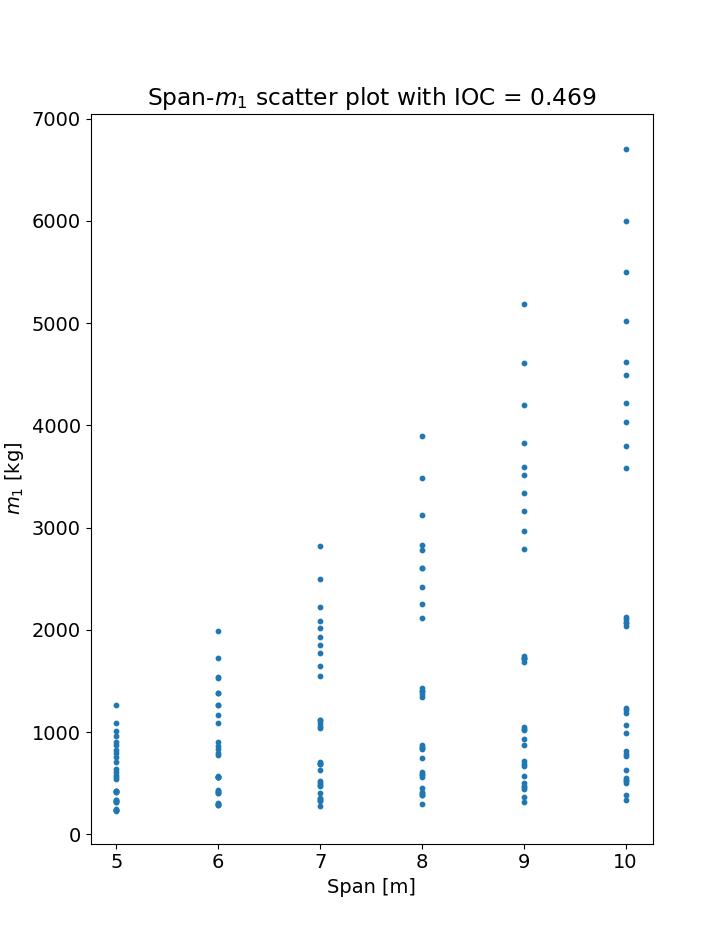
\includegraphics[width=.99\linewidth]{l_m1}
  \caption{$l-m_1$}
\end{subfigure}
~
\begin{subfigure}[b]{.32\textwidth}
  \centering
  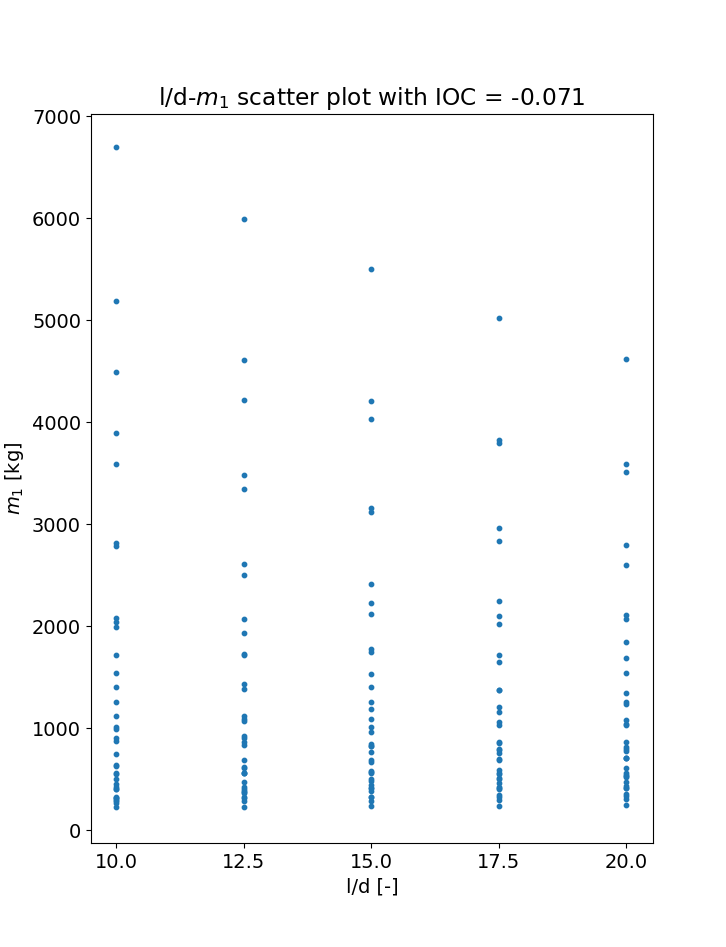
\includegraphics[width=.99\linewidth]{l2d_m1}
  \caption{$l/d-m_1$}
\end{subfigure}
~
\begin{subfigure}[b]{.32\textwidth}
  \centering
  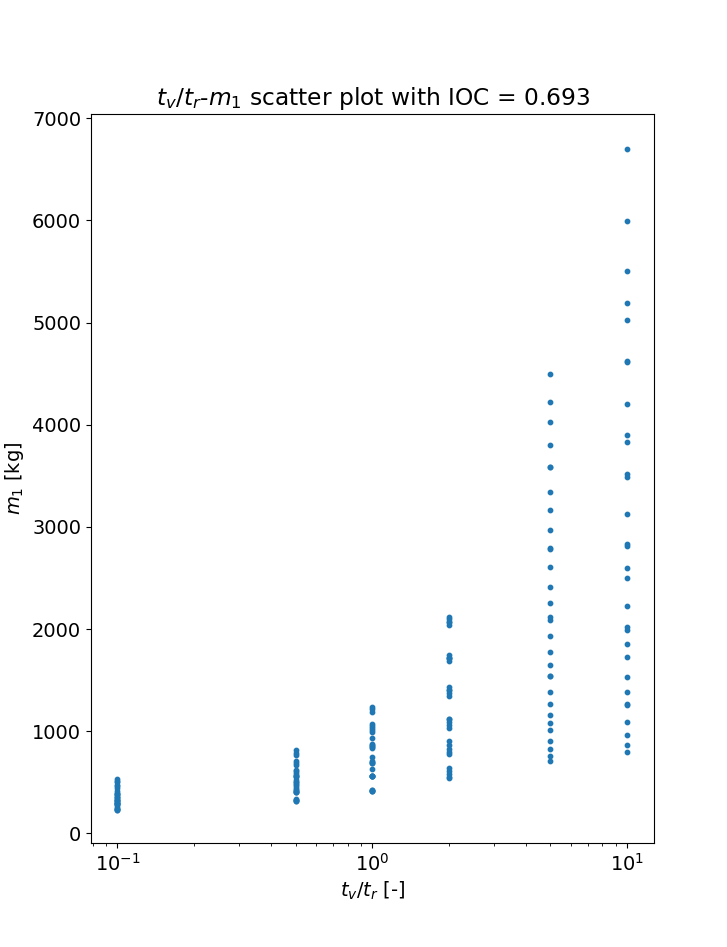
\includegraphics[width=.99\linewidth]{gamma_m1}
  \caption{$t_v/t_r-m_1$}
\end{subfigure}

\caption{Geometric parameters-modal mass (first mode) scatter plot}
\label{fig:geom-m1}
\end{figure}

\begin{figure}[H]
\centering
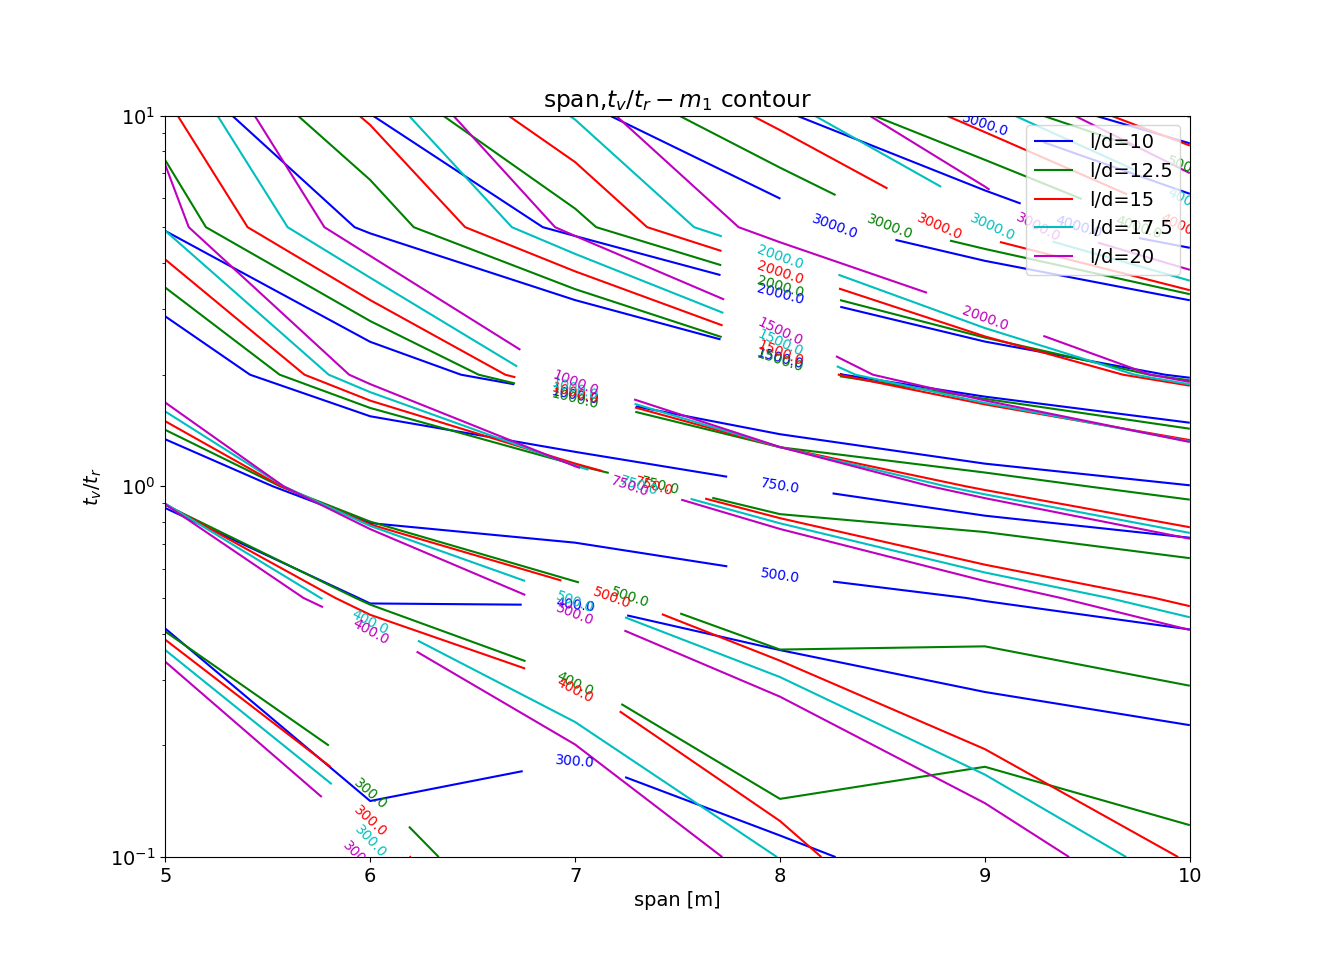
\includegraphics[width=0.9\textwidth]{images/l,gamma-m1.png}
\caption{$l, t_v/t_r - m_1$ contour plot}
\label{fig:l,t-m plot}
\end{figure}

It is interesting to see how the geometry changes the proportion of mass that participates in vibration, namely dimensionless quantity $m_1/m$ (see figure \ref{fig:geom-m12m}). Different from the modal mass, the modal mass proportion decreases with increasing span. It may be explained by the increasing number of ribs near the edges when span raises. The mass proportion of material in the middle becomes less, and the vertical vibration of the floor on the sides is likely to be restricted by the vertically stiff ribs, only allowing a small proportion of mass in the middle to vibrate. With increasing $l/d$ (thinner floor) the modal mass proportion goes up, which is shown more clearly in figure \ref{fig:m12m_change}. This may lie in a weaker arch effect if the vault is too shallow. The extreme is a flat floor without any arch effect leading to a modal mass of 25\% of total mass. The increase of $t_v/t_r$ promotes the modal mass proportion greatly. This is due to different mass and stiffness distribution in the vault and ribs. The vault has a more or less uniform mass distribution over the whole area, whereas the ribs have much higher mass and stiffness concentration around edges allowing only a small proportion of mass in the middle to vibrate. When the two different components work together, the vertically stiff ribs near edges are prone to impose constraints on the vault during vibration. 
No matter how these parameters change, the modal mass proportion can barely reach 13\%, it can be even lower than 0.5\% if ribs dominate. For floors with identical vault and ribs thickness, this value ranges from 1\% to 7\%, compared with flat slab with 25\%, the difference is huge.

\begin{figure}[H]
\begin{subfigure}[b]{.32\textwidth}
  \centering
  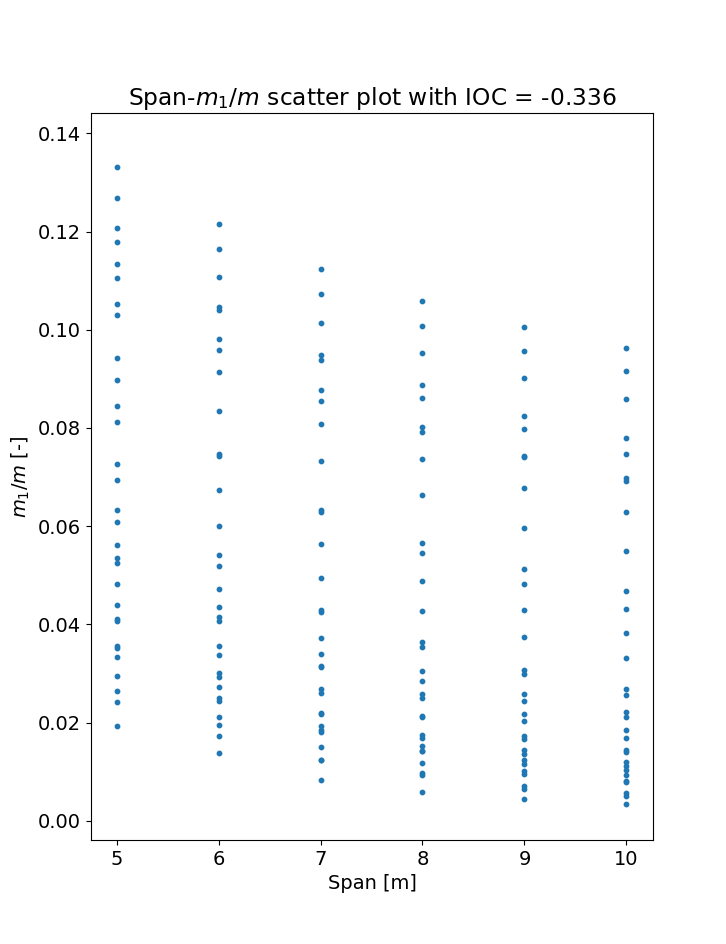
\includegraphics[width=.99\linewidth]{l_m12m}
  \caption{$l-m_1/m$}
\end{subfigure}
~
\begin{subfigure}[b]{.32\textwidth}
  \centering
  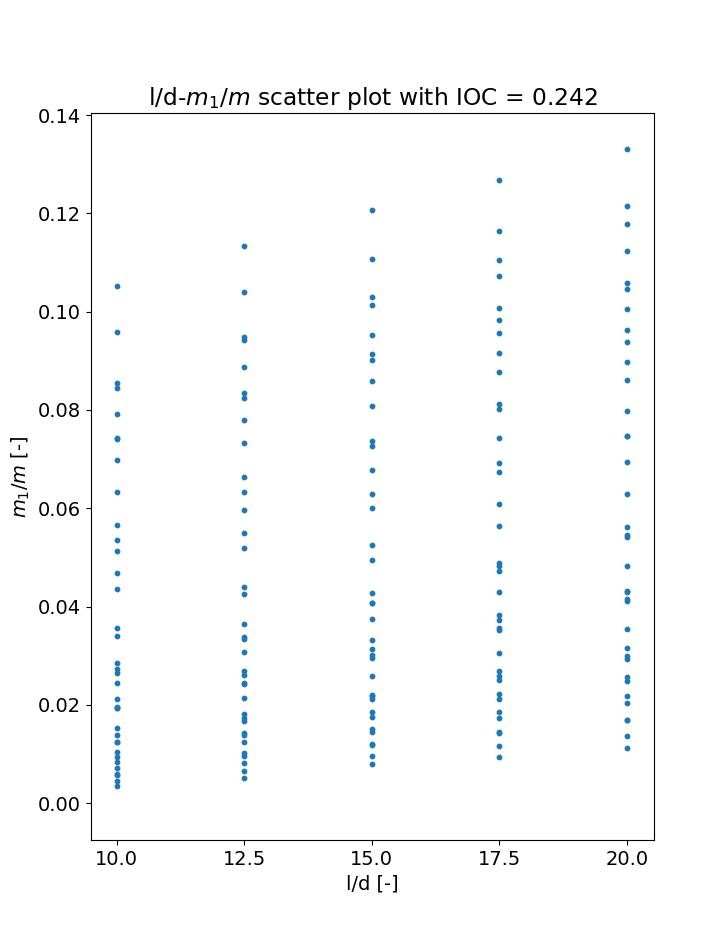
\includegraphics[width=.99\linewidth]{l2d_m12m}
  \caption{$l/d-m_1/m$}
\end{subfigure}
~
\begin{subfigure}[b]{.32\textwidth}
  \centering
  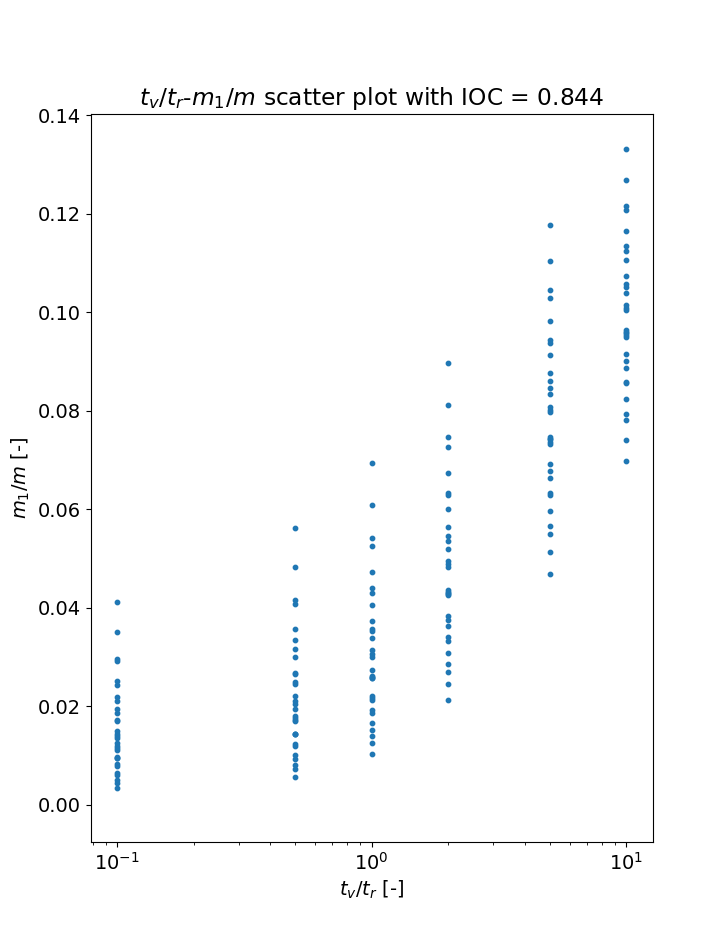
\includegraphics[width=.99\linewidth]{gamma_m12m}
  \caption{$t_v/t_r-m_1/m$}
\end{subfigure}

\caption{Geometric parameters-modal mass (first mode) proportion scatter plot}
\label{fig:geom-m12m}
\end{figure}

\begin{figure}
  \centering
  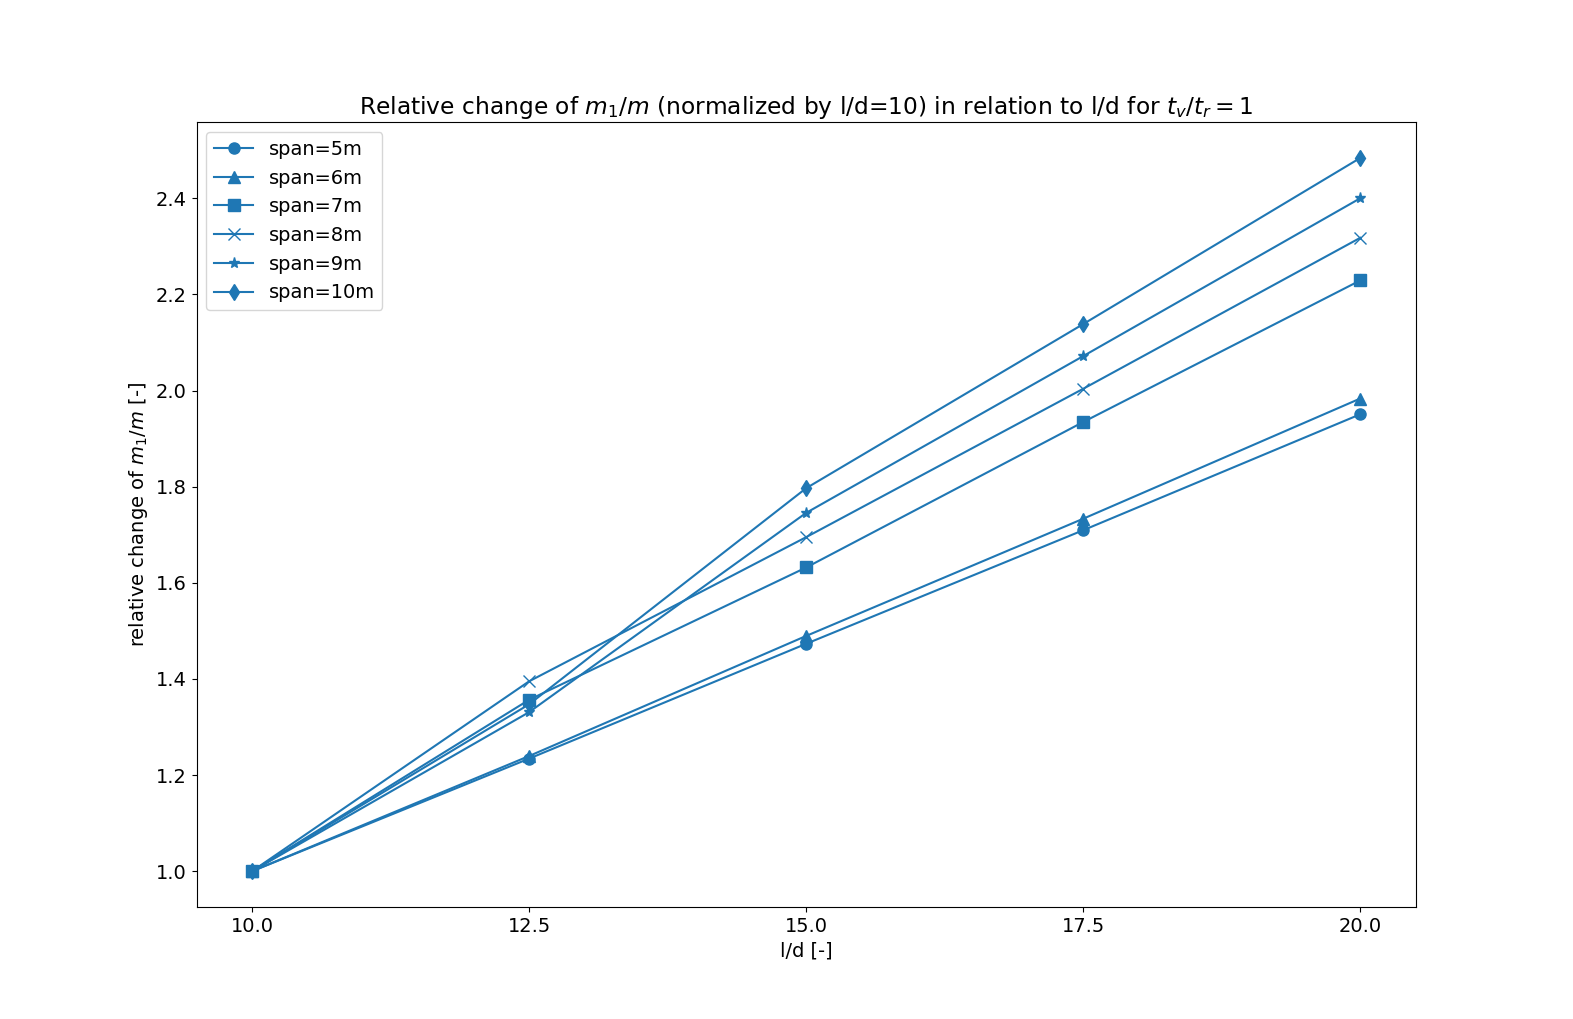
\includegraphics[width=0.9\linewidth]{images/m12m_change}
  \caption{Relative change of $m_1/m$ in relation to l/d}
  \label{fig:m12m_change}
\end{figure}

\subsection{Natural frequency}
\label{subsec:natural frequency}
The relation between natural frequency $f_n$ and angular frequency $\omega_n$ is $f_n=\omega_n/(2\pi)$. It is an important quantify for both low frequency floor as well as high frequency floor. For low frequency floor,it may be associated with the resonant behavior. For high frequency floor, it is the frequency at which the floor vibrates in the transient phase, instead of vibrating at the excitation frequency in the steady phase. The natural frequency is also involved in evaluation of vibration perception by the frequency weighting function. Figure \ref{fig:geom-f1} illustrates how $l, l/d, t_v/t_r$ influences the fundamental frequency (the first natural frequency). 
\begin{figure}[H]
\begin{subfigure}[b]{.32\textwidth}
  \centering
  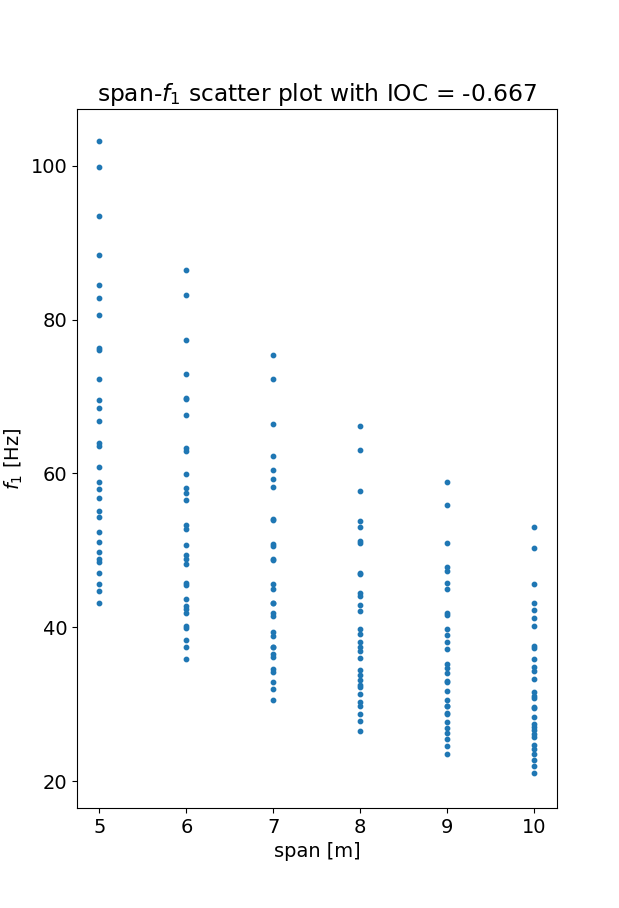
\includegraphics[width=.99\linewidth]{l_f1}
  \caption{$l-f_1$}
\end{subfigure}
~
\begin{subfigure}[b]{.32\textwidth}
  \centering
  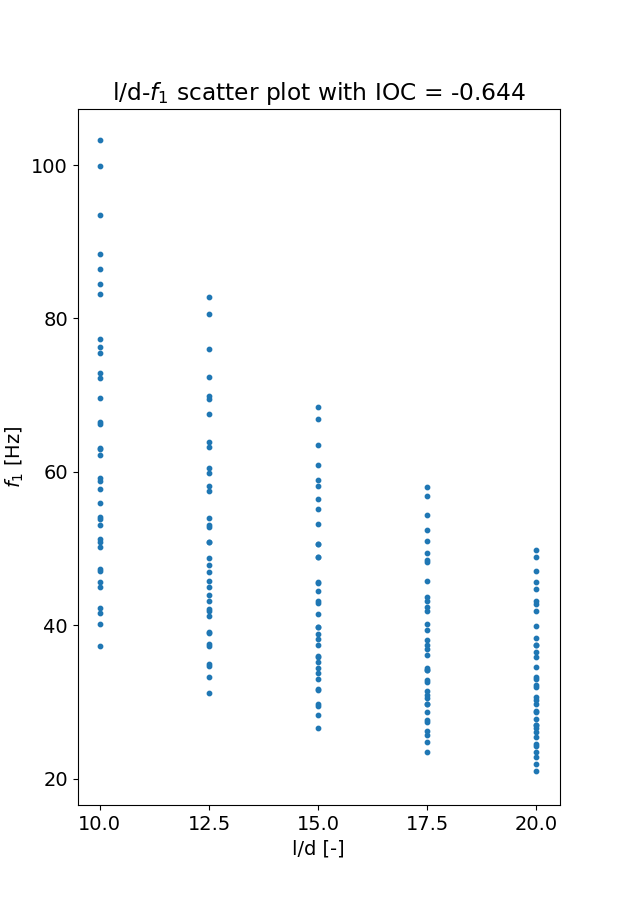
\includegraphics[width=.99\linewidth]{l2d_f1}
  \caption{$l/d-f_1$}
\end{subfigure}
~
\begin{subfigure}[b]{.32\textwidth}
  \centering
  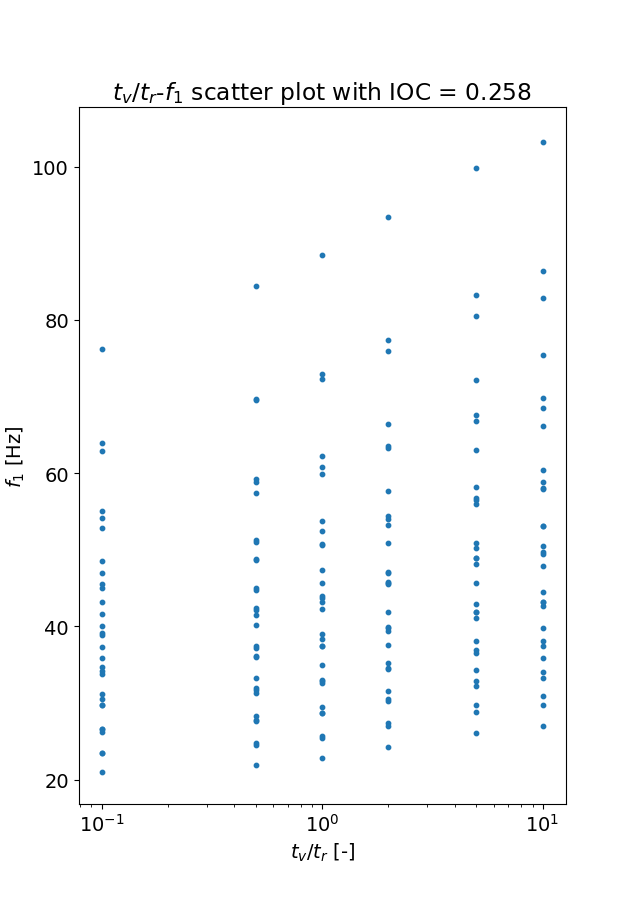
\includegraphics[width=.99\linewidth]{gamma_f1}
  \caption{$t_v/t_r-f_1$}
\end{subfigure}

\caption{Geometric parameters-natural frequency (first mode) scatter plot}
\label{fig:geom-f1}
\end{figure} 

It is interesting to observe that the natural frequency drops with increasing span. As span is the only index in the three geometric parameters that has a unit, a concrete number, instead of a dimensionless ratio that represents a scalable model. Plot (a) indicates that the natural frequency has a size effect, the bigger the size is, the lower natural frequency it shows. An increase in $l/d$ results in an reduction in frequency as the arch effect is weaker. The $t_v/t_r$ ratio does not influence the natural frequency much (with slightly positive effect), which can be explained by $\omega_n=\sqrt{k/m}$. For the vault, k and m are roughly evenly distributed everywhere, for the ribs, where there is less mass also shows less stiffness, so the ratio can keep more or less the same. 

Figure \ref{fig:m1_f1} shows the $m_1-f_1$ scatter plot, there exists no clear correlation between the two modal parameters.

\begin{figure}[H]
\centering
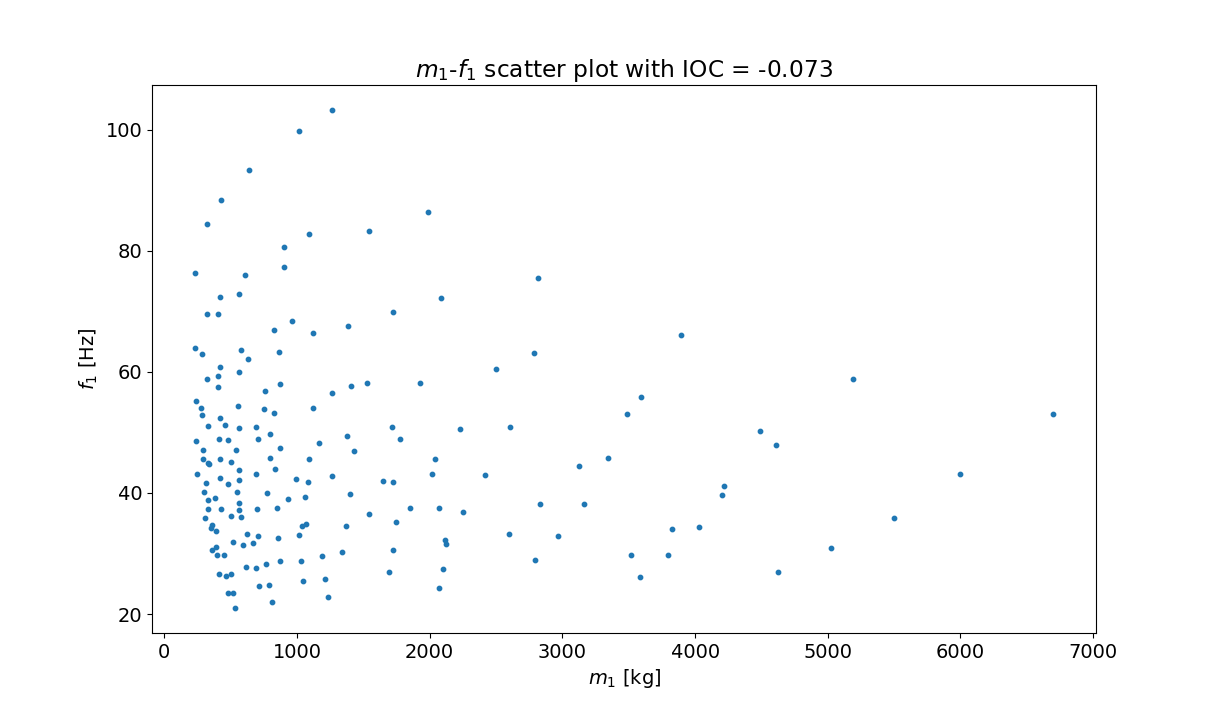
\includegraphics[width=1\textwidth]{images/m1_f1}
\caption{$m_1 - f_1$ scatter plot}
\label{fig:m1_f1}
\end{figure}


\subsection{Mode shape}
All floors show similar first 6 mode shapes as illustrated in figure \ref{fig:mode_shapes}. As stated above, the $t_v/t_r$ ratio influences the area involved in vibration. The ribs tend to restrict the vibration in a smaller region in the middle and impose constraint on the vault near edges. It also can be described from another side, the vault tens to disperse the vibration to a larger region, figure \ref{fig:first_modes} is the demonstration. When the vault dominates, the region with large vibration amplitude expands compared to a ribs dominating floor.
\begin{figure}[H]
\centering
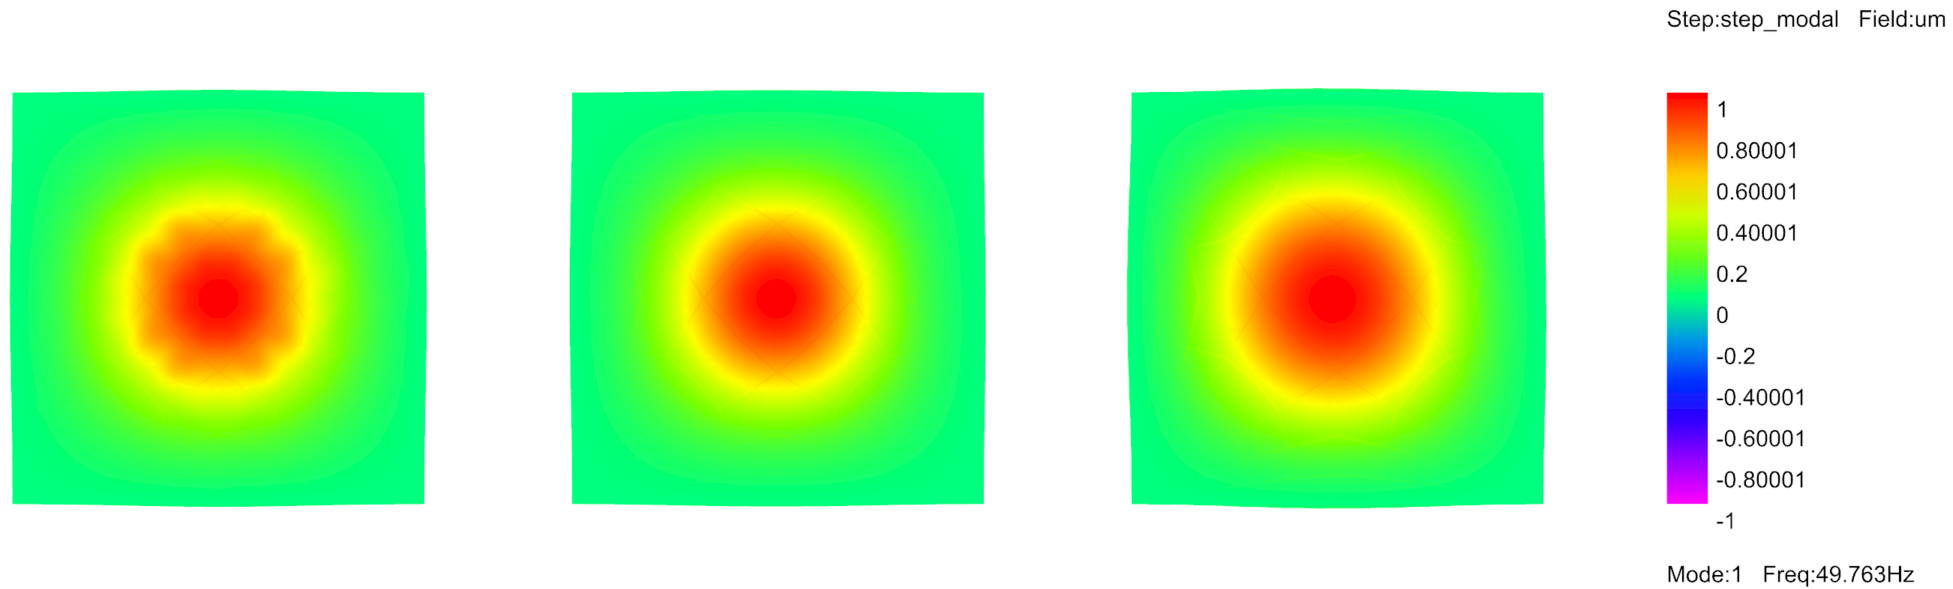
\includegraphics[width=1\textwidth]{images/first_modes}
\caption{first mode shapes with $t_v/t_r=0.1,1,10$ from left to right}
\label{fig:first_modes}
\end{figure}

\section{Solution of response time history}
The theoretical background and solving procedure have been described in section \ref{subsec:modal_superposition} and \ref{subsec:resp_time_histroy}. The equation of motion in modal coordinate and the response time history via modal superposition were solved based on equation \ref{eqn:motion_q} and \ref{eqn:u} in Python. It is very necessary to compare the results from Python with those from Abaqus for calibration.
\subsection{Modeling in Abaqus}
An Abaqus model of a floor with $l=5m, l/d=20, t_v/t_r=1$ was built. This model is imported from the Rhino mesh model, so the models for Abaqus and for Python are exactly the same, except for the definition of damping. In Python, the damping ratio $\xi=3\%$ is defined for all modes, as it is a feature of a mode. In Abaqus, however, the definition of damping is executed in material module. For the Rayleigh damping, the damping matrix consists of the mass-proportional damping and the stiffness-proportional damping,
\begin{equation}
    \mathbf{c}=\alpha\mathbf{m}+\beta\mathbf{k}
\end{equation}
\noindent
where $\alpha$ represents the mass coefficient and $\beta$ the stiffness coefficient. The damping ratio related to each mode varies along with the angular frequency (as shown in figure \ref{fig:damping}):
\begin{equation}
    \xi_n=\frac{\alpha}{2\omega_n}+\frac{\beta\omega_n}{2}
\end{equation}
\noindent
To solve $\alpha$ and $\beta$, damping ratios from two modes $i, j$ are needed. The damping ratio of modes in between will be underestimated, while outside of the range overestimated. The damping ratio of the first mode should be precisely set to be 3\%. If the other mode is the 2nd mode, damping ratios of all later modes will be overestimated. The choice of the mode $j$ is model dependent, it hinges on the complexity (number of DOFs) of the model and number of modes that effectively participate in vibration. Considering that this mesh model has 13211 elements and the first 25 modes may be effectively involved in vibration, the damping ratio of the 10th mode is set to be $3\%$. Then the calculated $\alpha$ and $\beta$ were given in Abaqus, and a calculation with standard (implicit) solver for dynamics was launched.
\begin{figure}[H]
\centering
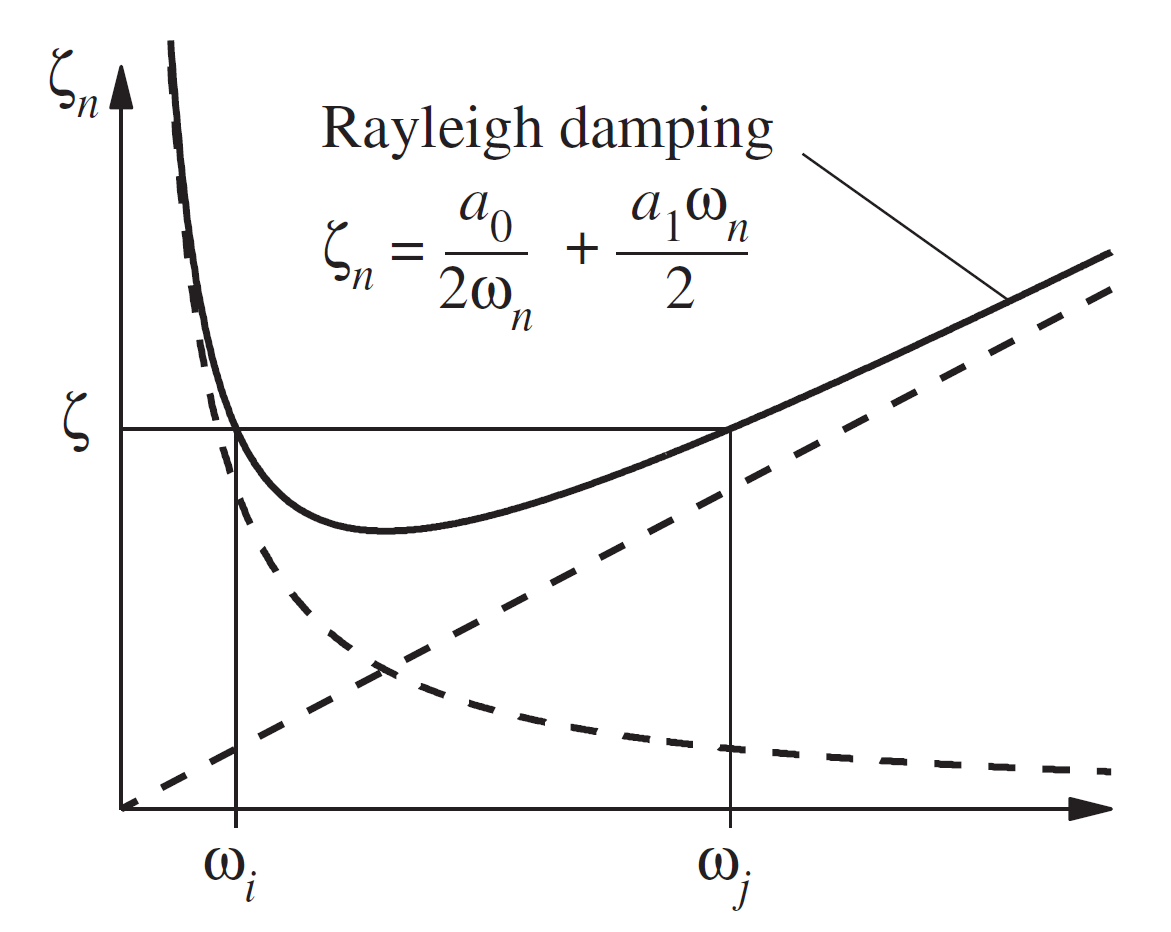
\includegraphics[width=0.5\textwidth]{images/damping}
\caption{Damping ratio in relation to angular frequency \cite{chopra2007dynamics} with notation $a_0=\alpha$, $a_1=\beta$ }
\label{fig:damping}
\end{figure}
\subsection{Calibration of results with Abaqus}
The results of response time history analysis from Abaqus and Python are compared in figure \ref{fig:response_abq}. 100 modes are used for modal superposition, and the contribution of the first mode is also plotted. It shows a very good match of the data. The results from modal superposition present a slightly lower value in displacement, which is reasonable as not all modes have involved. Then they show a slightly higher value in acceleration and rms-acceleration, suggesting a conservative evaluation. Such response indicates a very typical transient phase, where the structure vibrates at its natural frequencies right after the excitation and the energy dissipates quickly through damping. Afterwards, the structure will calm down and step into the steady phase, where the vibration continues but at the excitation frequency. The peak of rms-acceleration always appears at the first moment when it is calculated, namely at 0.5s, in all studied floors.

\begin{figure}[H]
\centering
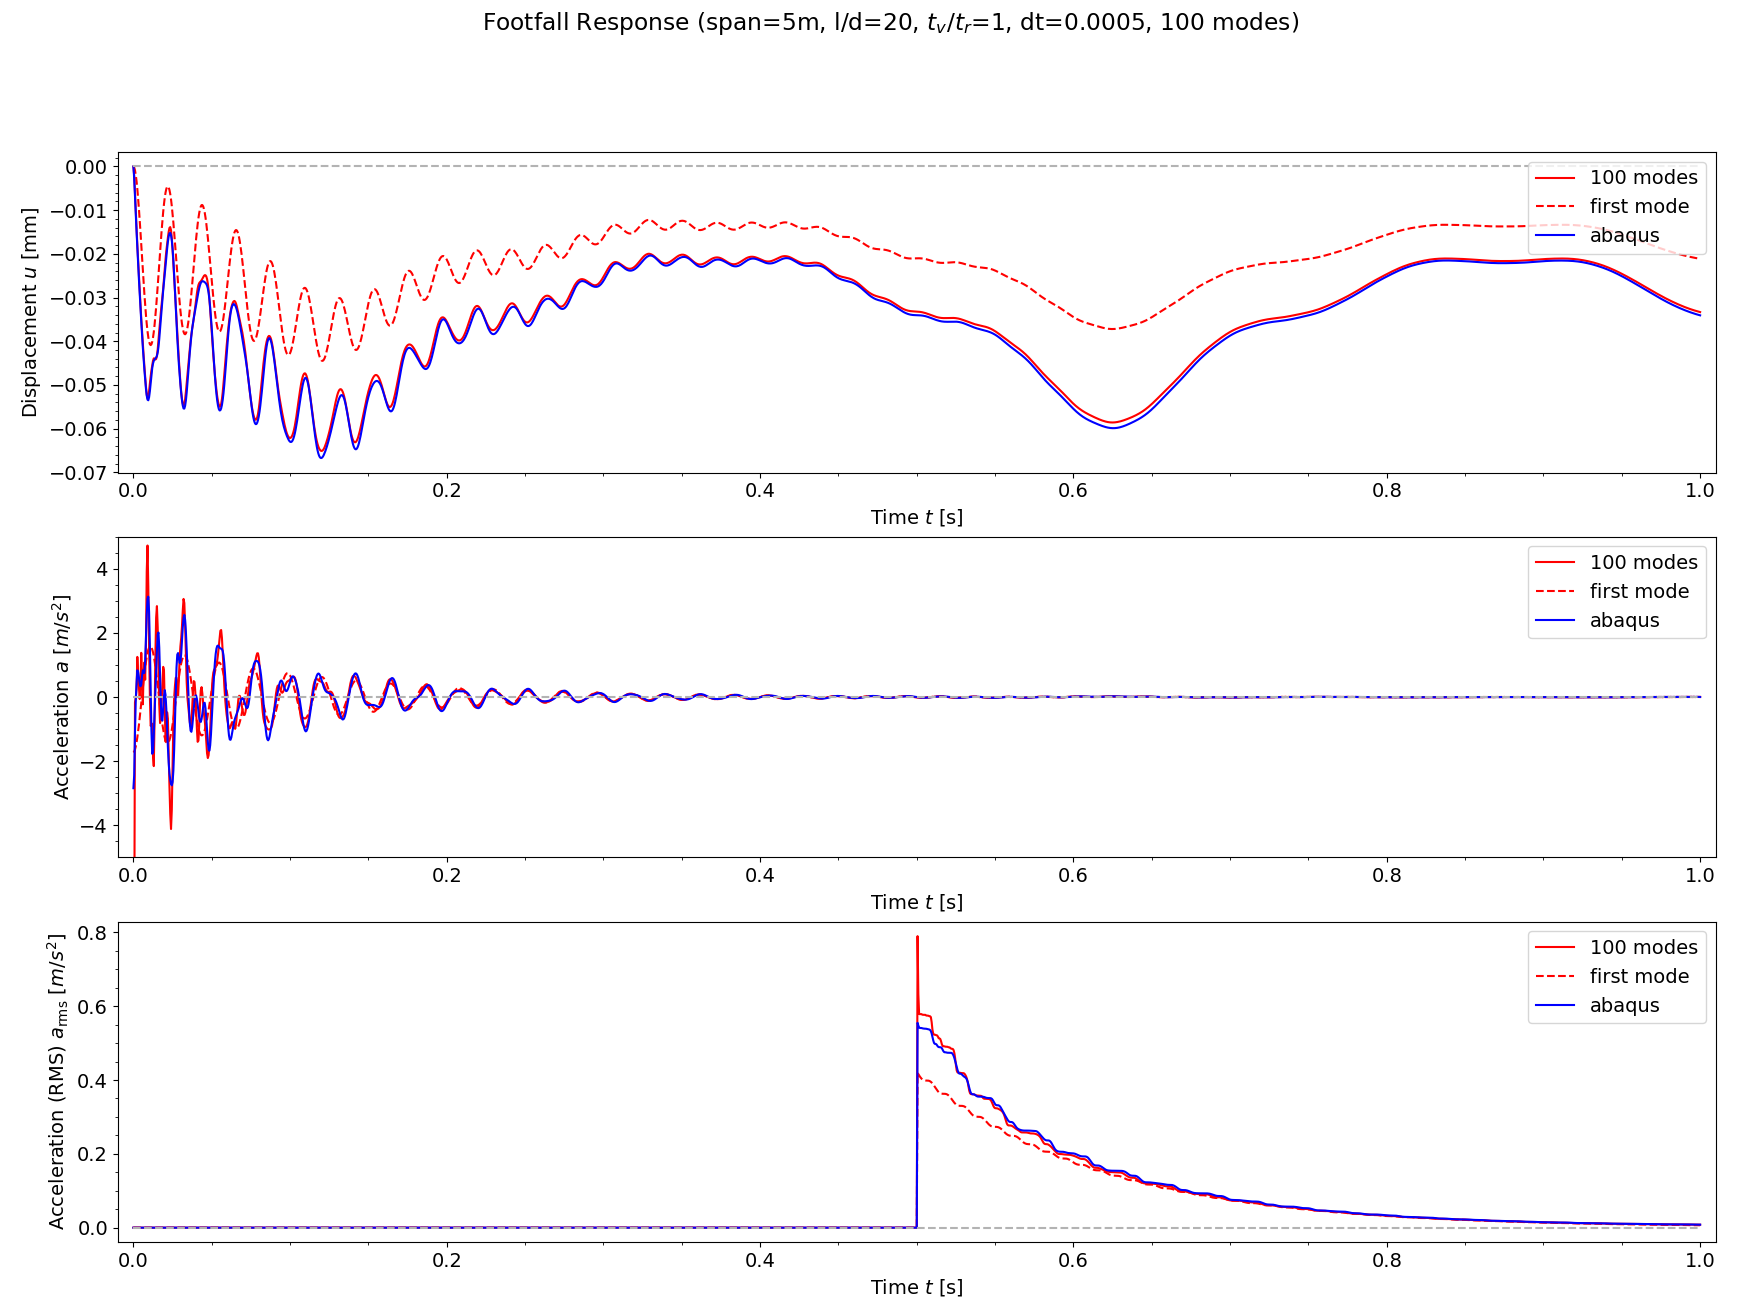
\includegraphics[width=1\textwidth]{images/response_abq.png}
\caption{Comparison of footfall response calculated by Abaqus and by Python with modal superposition}
\label{fig:response_abq}
\end{figure}

This plot also indicates that the first mode is not enough to represent the displacement or acceleration. In addition, there appears a peak in rms-acceleration that derives from an unrealistically high acceleration that is no shown in the acceleration subplot. The complete picture of the subplot is shown in figure \ref{fig:acc_whole}. This unrealistic value takes place at the first calculation time interval, and it stems from the derivation of velocities in high modes. These problems will be fixed to a large degree when the frequency weighting takes part in the evaluation. 
\begin{figure}[H]
\centering
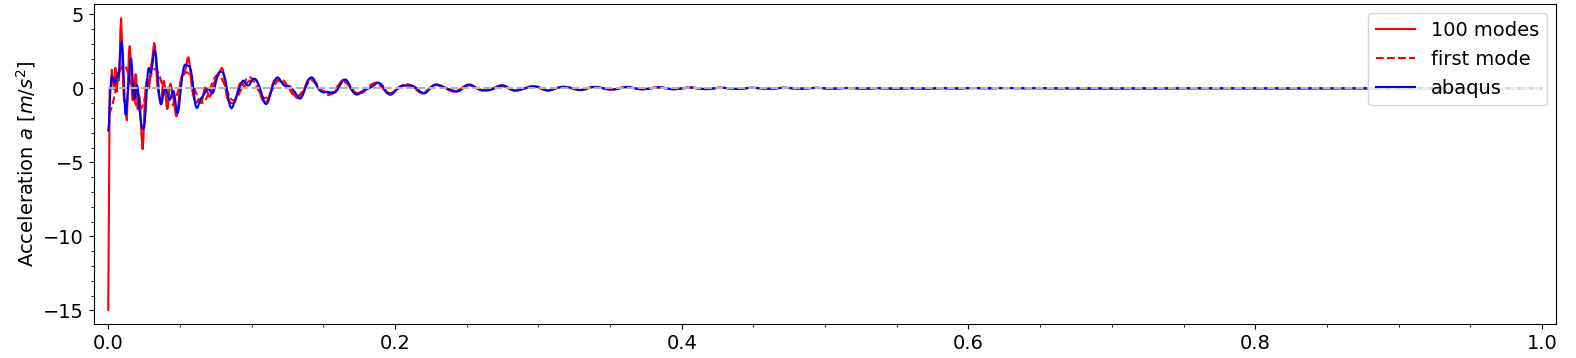
\includegraphics[width=1\textwidth]{images/acc_whole}
\caption{The whole picture of acceleration with extreme value}
\label{fig:acc_whole}
\end{figure}

\subsection{Frequency weighted response}
Note that for the rms-acceleration subplot in figure \ref{fig:response_abq}, the frequency weighting is not introduced.Figure \ref{fig:acc_weight} shows both the original and weighted rms-acceleration. It is clear that the frequency weighting plays a very important role by reducing the response by 70\% for this floor. It also can be seen that the response from the first mode can represent the total response quite well, more than 88\% of the total response is contributed by the first mode. Moreover, the frequency weighting has a peak clipping effect by filtering out the response from high modes.

\begin{figure}[H]
\centering
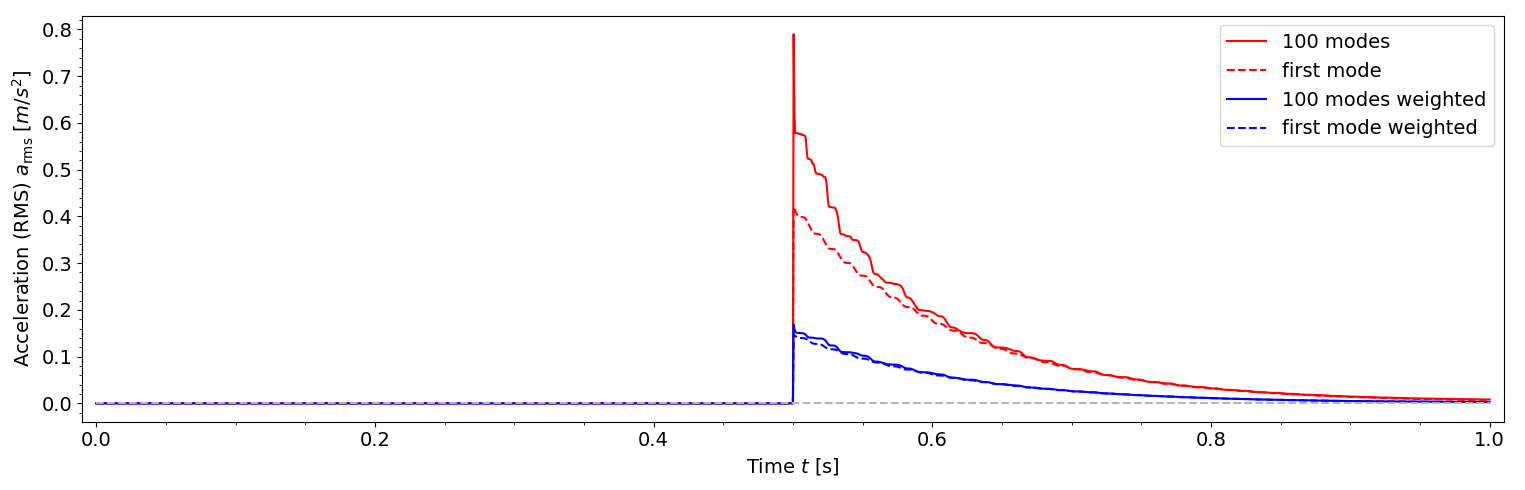
\includegraphics[width=1\textwidth]{images/acc_weight}
\caption{Original and weighted rms-acceleration}
\label{fig:acc_weight}
\end{figure}

\subsection{Number of modes for modal superposition}
One important issue in solution of the response is the proper number of modes for superposition. On the one hand, it can not be too few so that the response loses its accuracy. On the other hand, it should not be too high so that the computation becomes unaffordable or uneconomic. The recognition of important modes then become significant. Some modes are more effectively activated than others, they tend to (but not necessarily) contribute more in the total response. 

Figure \ref{fig:res_part_factor} shows the unweighted and weighted response factor as well as participation factor in relation to modes involved in modal superposition. Again, the figure illustrates the significance of frequency weighting. The unweighted response factor continues increasing even when 100 modes are adopted, whereas the weighted response factor shows a plateau after 30 modes. The modal participation factor is a modal parameter that indicates whether a mode is effectively activated or not. It is formulated in equation \ref{eqn:Gamma} and repeated here for convenience:
\begin{equation}
    \label{eqn:Gamma_1}
    \Gamma_n=\frac{\boldsymbol{\phi}_n^T\mathbf{s}}{M_n}
\end{equation}
\noindent
It is further used for the calculation of modal load
\begin{equation}
    P_n(t)=\Gamma_nP(t)
\end{equation}
\noindent
Only when the mode shape $\boldsymbol{\phi}$ and spatial distribution vector \textbf{s} are in alignment with each other, a large participation factor, namely a considerable load will be applied on this mode. Where there is a high participation factor, there appears an increase in response factor, although to different degrees. Several modes that are effectively activated (mode 1,6,11,15) and not activated (mode 23) are listed for visualization and comparison. For mode 11, because the largest displacement is not in the middle, so the middle point is not normalized as 1 but a negative value, resulting in a negative participation factor with less magnitude.

\begin{figure}[H]
\centering
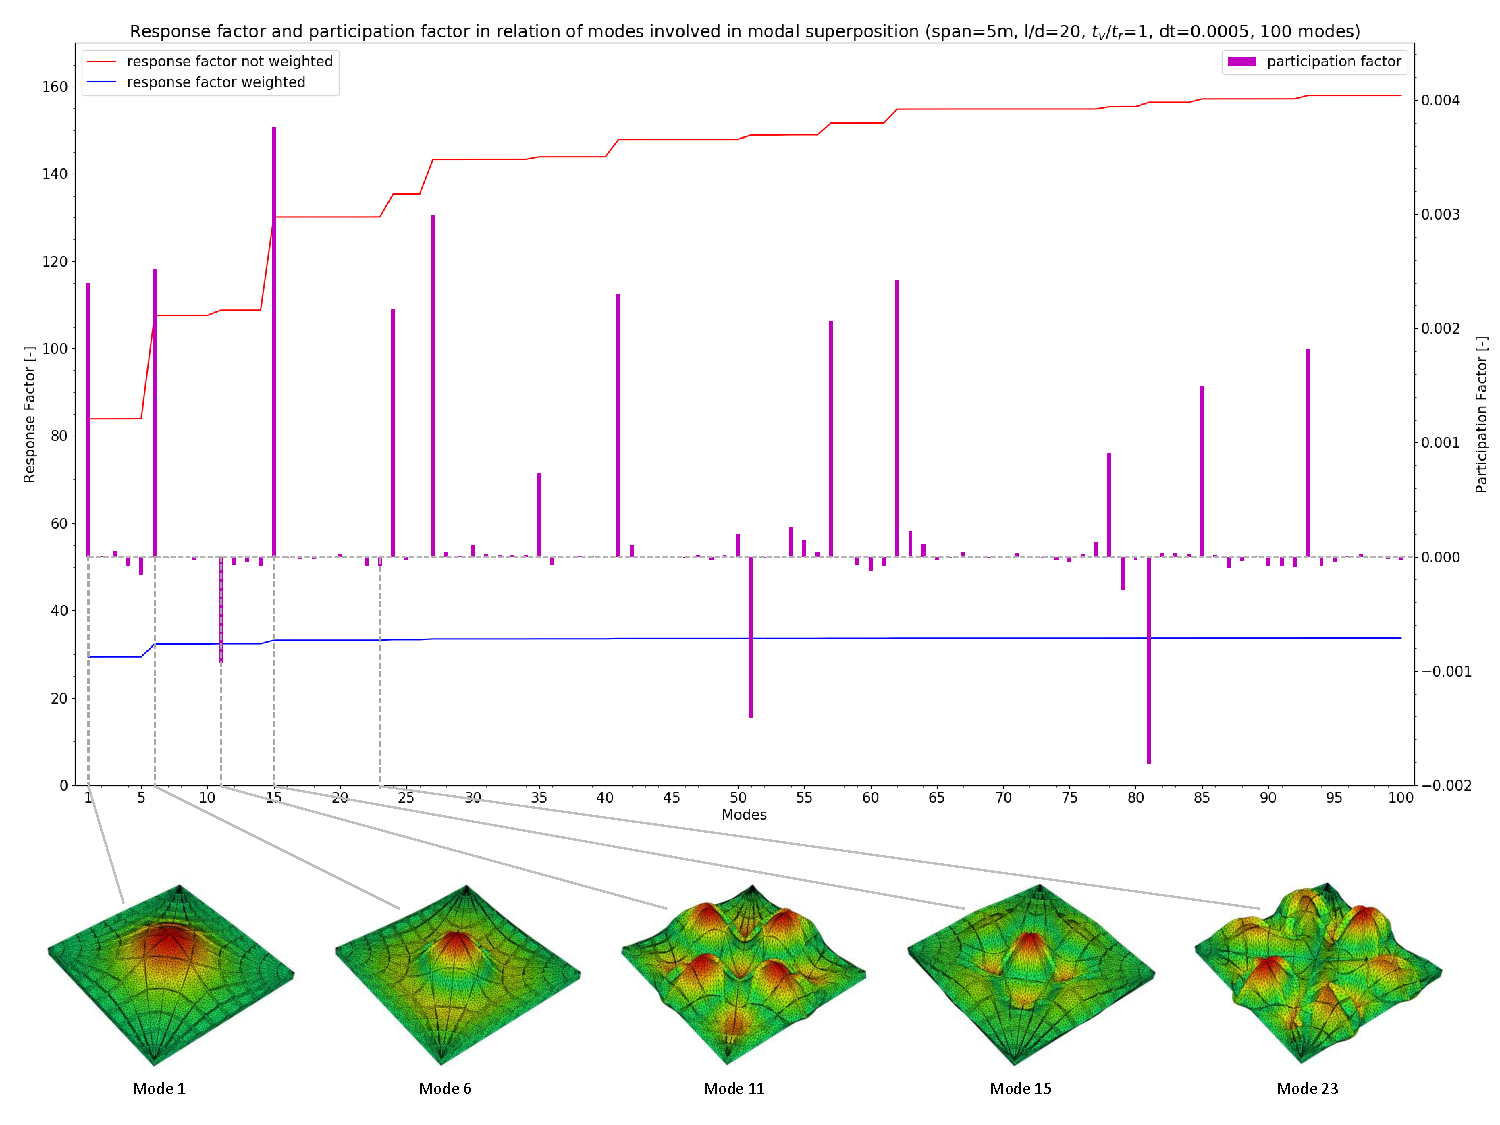
\includegraphics[width=1\textwidth]{images/res_part_factor.pdf}
\caption{Response factor and participation factor in relation to modes involved in modal superposition}
\label{fig:res_part_factor}
\end{figure}

It is worth mentioning that the modal participation factor does not imply the actual contribution of the mode to the total response. Because to solve the equation of motion in modal coordinates
\begin{equation}
\ddot{q_n}+2\xi_n\omega_n\dot{q_n}+\omega_n^2q_n=\Gamma_nP(t)
\label{eqn:motion_q_1}
\end{equation}
\noindent   
damping ratio $\xi_n$ and angular frequency $\omega_n$ also play a role. Given that the damping ratio holds the same for all modes, a higher angular frequency will result in a lower solution of the modal coordinate. That's the reason why even with similar participation factors, higher modes tend to contribute less than lower modes. An objective indicator of the actual contribution would be modal contribution factor, which is defined as the ratio of response associated with certain mode to the total response
\begin{equation}
    \Bar{r}_n=\frac{r_n}{r}
\end{equation}
\noindent
The contribution factor shown in figure \ref{fig:contr_factor} indicates that the unweighted response has more contribution from modes other than the first mode, while the weighted response heavily relies in the first mode. Generally, the contribution of the first mode to the weighted response varies from 86\% to 92\% for all studied floor models, therefore the response from the first mode is a good indicator of the total response.  
\begin{figure}[H]
\centering
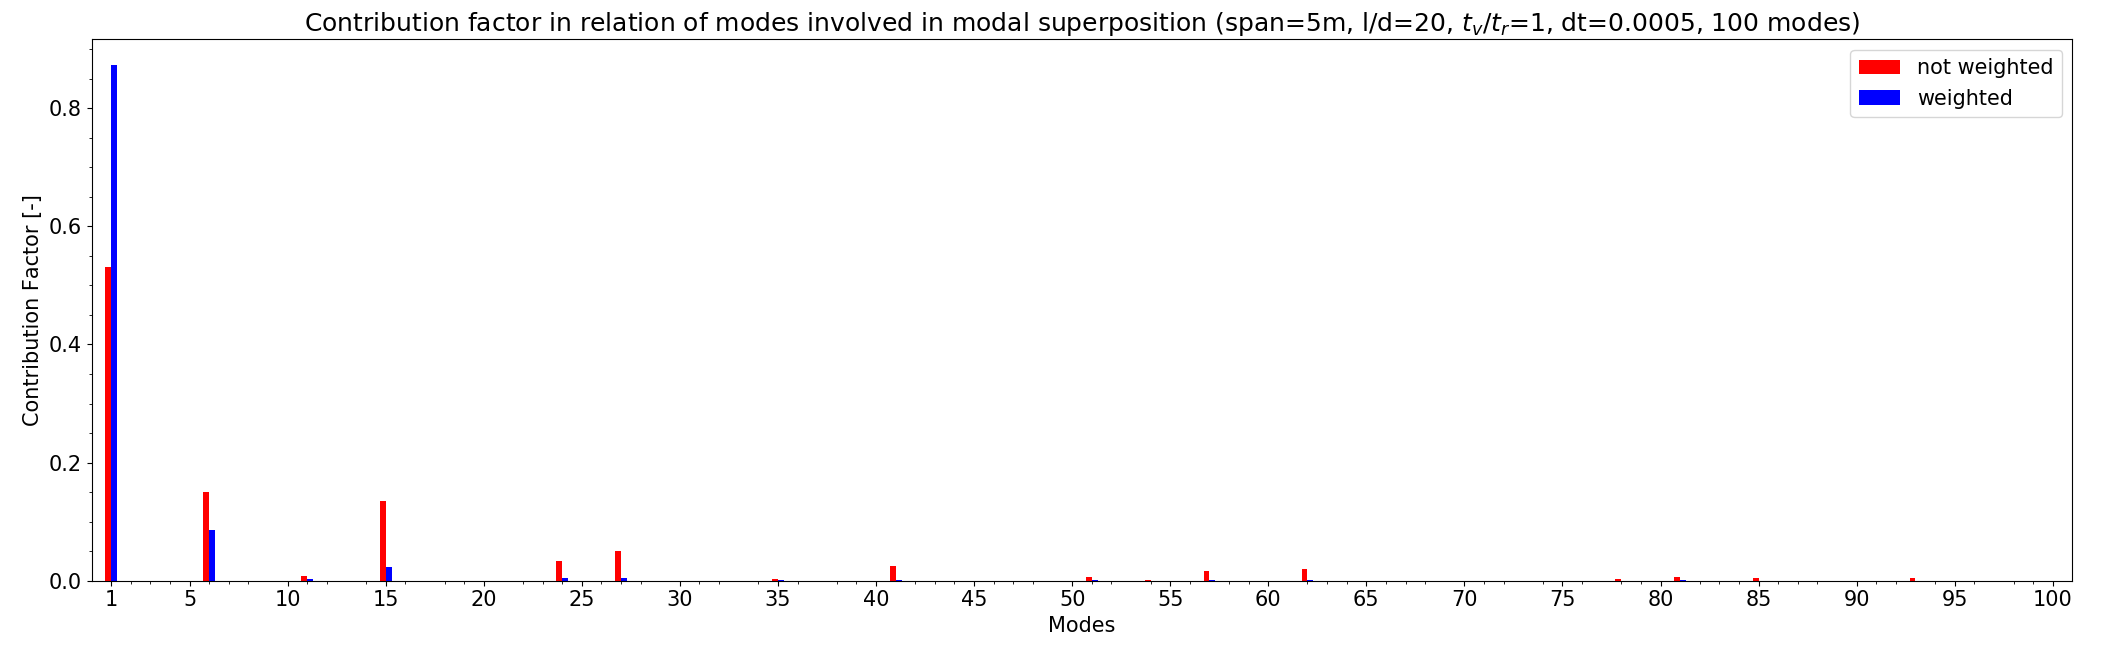
\includegraphics[width=1\textwidth]{images/contr_factor}
\caption{Contribution factor in relation to modes involved in modal superposition}
\label{fig:contr_factor}
\end{figure}

Although the weighted response factor keeps almost unchanged after 30 modes for the floor with $l=5m, l/d=20, t_v/t_r=1$, 50 modes are used for the calculation of all floors. The reason is that this floor has a fundamental frequency of $f_1=76$ Hz, which leads to a very strong frequency weighting effect. There are also some other floors with fundamental frequencies as low as 20 Hz that need more modes for superposition, because responses from high modes cannot be effectively filtered out and they will make considerable contribution to the total response.

\subsection{Advantages of modal superposition}
The implementation of response time history analysis via modal superposition in Python, instead of directly using existing FEM software like Abaqus, has the following advantages:
\begin{itemize}
    \item Much faster than Abaqus standard solver for dynamics. For the floor shown above, the smallest one among all floors, Abaqus took almost 2 hours, while the modal analysis in Abaqus and modal superposition in Python together took around 6 min for 100 modes, 4 min for 50 modes.
    \item Possibility of access to each mode, which is crucial for the post-process of the original response, for example frequency weighting. Abaqus has also modal superposition based dynamic solver, which took almost the same time as Python. It does not, however, provide the possibility to access to each mode, or only possible in a cumbersome way. 
    \item More structural insight into the its dynamic behavior. The solution of the response time history is no longer a black box, but a transparent one in which the correlation among parameters can be explained and checked.
\end{itemize}


\section{Evaluation of dynamic performance}
\subsection{Influence of geometric parameters}
The dynamic performance of the 180 floors with all different $l,l/d,t_v/t_r$ combinations were evaluated. The dynamic performance is characterized by the weighted response factor (called response factor later in the text and R in plots for simplicity). 
Figure \ref{fig:geom-R_contour} shows the influence of the geometric parameters on the response factor. In each subfigure the $l/d,t_v/t_r-R$ contour lines of a certain span are plotted. Take span=5m for example, the contour lines are smooth, the contour of response factor ranges from 4.0 to 56.0. The response increases in the positive direction of $l/d$ axis and negative direction of $t_v/t_r$ axis, which means a shallow and ribs dominating floor will have a large dynamic response. This observation matches with previous conclusion associated with modal mass and natural frequency in section \ref{subsec:modal_mass} and \ref{subsec:natural frequency}. The $l/d$ ratio does not influence modal mass much, but a high $l/d$ implies a low natural frequency, which results in a less pronounced frequency weighting effect and consequently a higher response factor. The $t_v/t_r$ ratio, on the contrary, shows an obvious positive correlation with the modal mass but almost no influence on the natural frequency. A lower $t_v/t_r$ value indicates a lower modal mass, which means that it is easier to get mobilized by a certain excitation based on the Newton's second law $a=F/m$. 

When the responses of different spans are compared, two trends can be observed: a wider range of response factor (especially the upper bound) and a less important role of $l/d$ with increasing span. The former can be explained by the dropping natural frequency along with larger span and the increase in modal mass cannot compensate it when the $t_v/t_r$ ratio is very low. The latter may lie in the concentration of ribs on the sides in large spans. The increase in natural frequency with a lower $l/d$ value is credited to a more fully developed arch effect. Since more mass is concentrated in ribs around the edges, the arch effect is weakened, so the $l/d$ value cannot influence the natural frequency much. More generally speaking, the natural frequency will not increase if the mass and stiffness distribution is not adequately optimized according to $\omega_n=\sqrt{k/m}$.

\begin{figure}
\begin{subfigure}[b]{.49\textwidth}
  \centering
  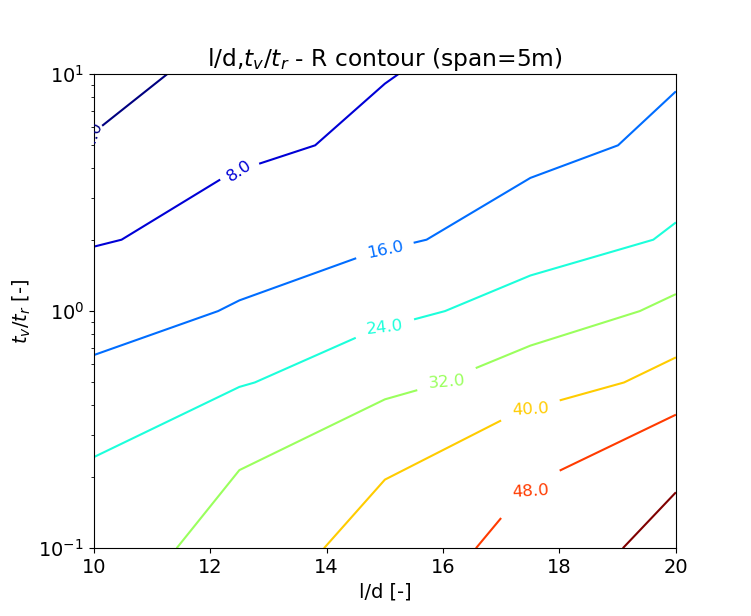
\includegraphics[width=.99\linewidth]{images/l2d,gamma_R_5m.png}
  \caption{span=5m}
\end{subfigure}
~
\begin{subfigure}[b]{.49\textwidth}
  \centering
  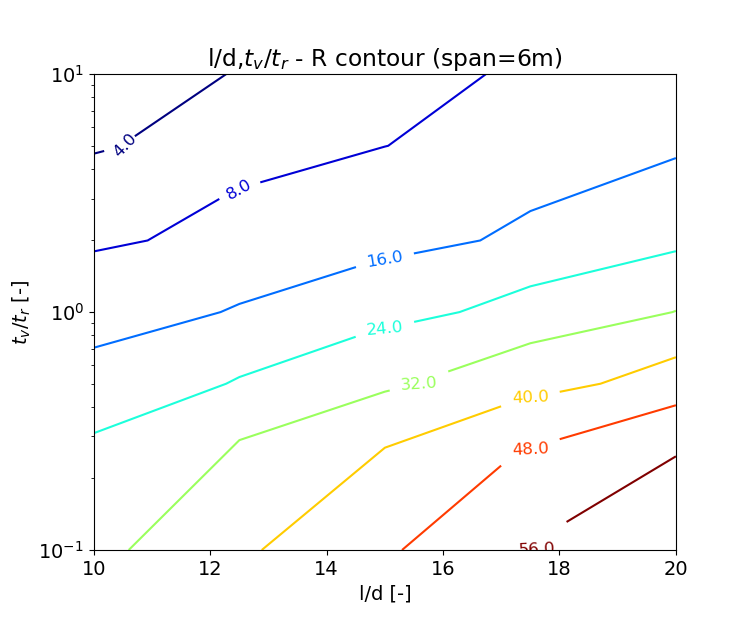
\includegraphics[width=.99\linewidth]{images/l2d,gamma_R_6m.png}
  \caption{span=6m}
\end{subfigure}

\begin{subfigure}[b]{.49\textwidth}
  \centering
  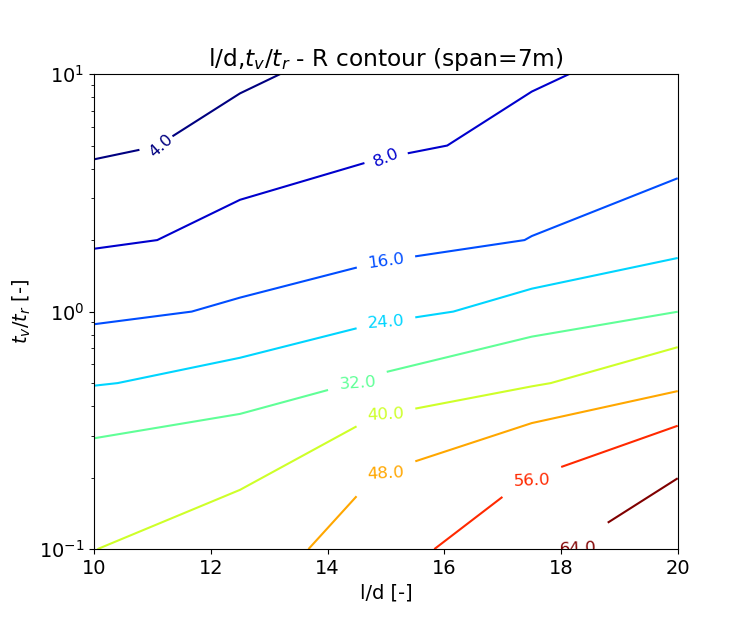
\includegraphics[width=.99\linewidth]{images/l2d,gamma_R_7m.png}
  \caption{span=7m}
\end{subfigure}
~
\begin{subfigure}[b]{.49\textwidth}
  \centering
  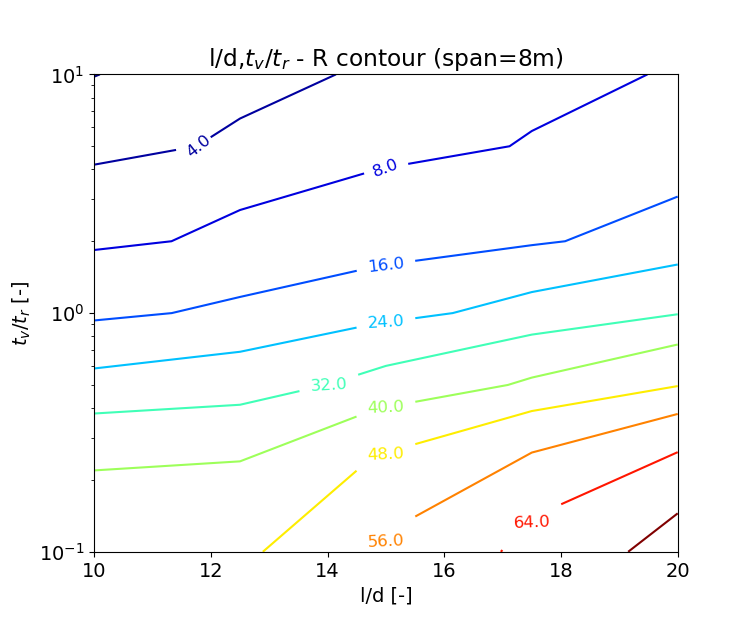
\includegraphics[width=.99\linewidth]{images/l2d,gamma_R_8m.png}
  \caption{span=8m}
\end{subfigure}

\begin{subfigure}[b]{.49\textwidth}
  \centering
  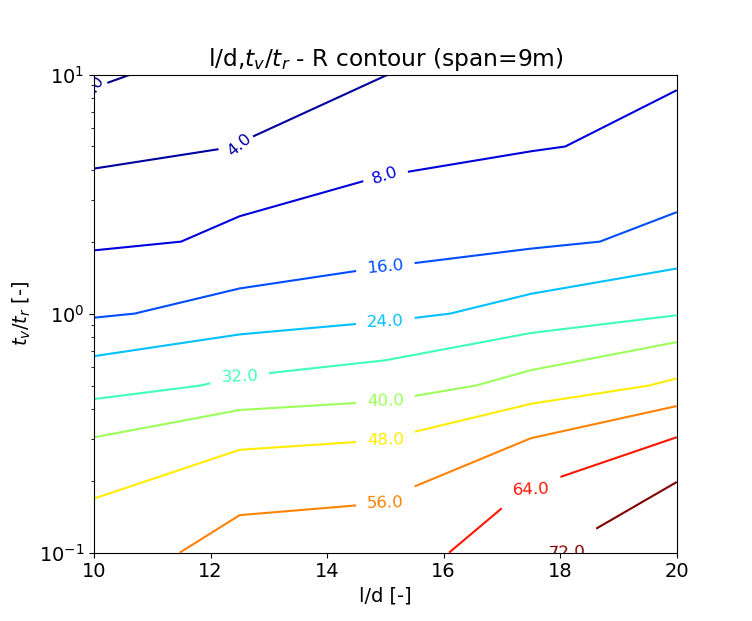
\includegraphics[width=.99\linewidth]{images/l2d,gamma_R_9m.png}
  \caption{span=9m}
\end{subfigure}
~
\begin{subfigure}[b]{.49\textwidth}
  \centering
  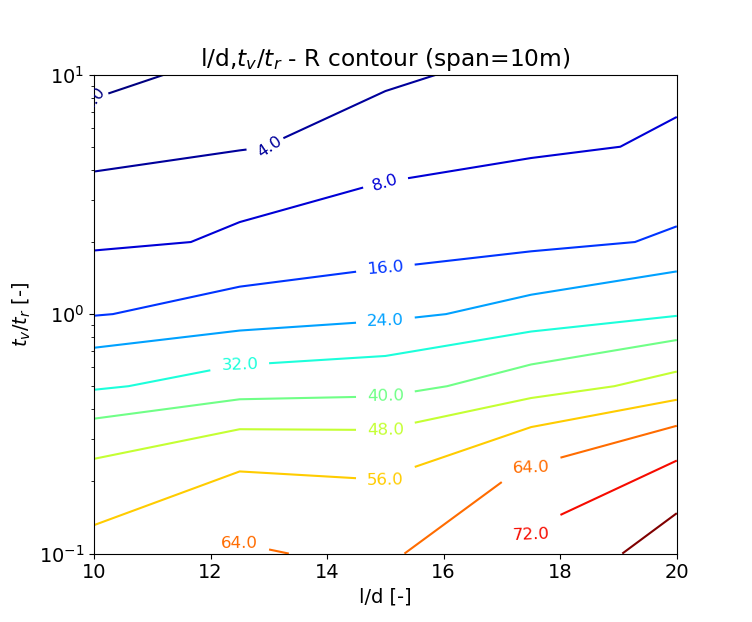
\includegraphics[width=.99\linewidth]{images/l2d,gamma_R_10m.png}
  \caption{span=10m}
\end{subfigure}

\caption{Geometric parameters-response factor contour plot}
\label{fig:geom-R_contour}
\end{figure} 

The relation between the geometric parameters and the response factor can also be depicted with input/output correlation scatter plot as shown in figure \ref{fig:geom-R_scatter}. It indicates that the span has very little influence on the dynamic performance, $l/d$ ratio has some importance and the $t_v/t_r$ has the greatest significance. This importance sequence conforms well to the decision-making power of engineers. Floors with different spans, which are usually not determined by engineers, can behave equally well or badly. $l/d$ ratio, in which engineers may participate in the decision, can have some influence on the dynamic behaviour. Through $t_v/t_r$ ratio, which can be decided by engineers to a large extent, the dynamic performance can be greatly altered (optimized if in a good way). Of course, such coincidence is valid only under the given pattern and scaling scheme.

\begin{figure}[H]
\begin{subfigure}[b]{.32\textwidth}
  \centering
  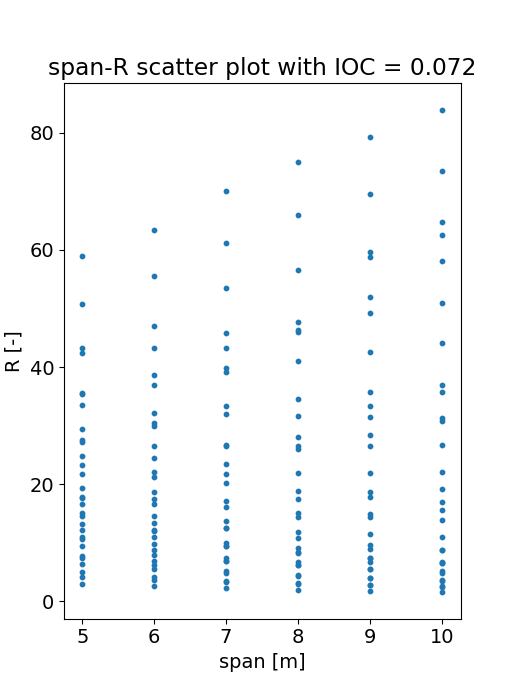
\includegraphics[width=.99\linewidth]{span_R}
  \caption{$l-R$}
\end{subfigure}
~
\begin{subfigure}[b]{.32\textwidth}
  \centering
  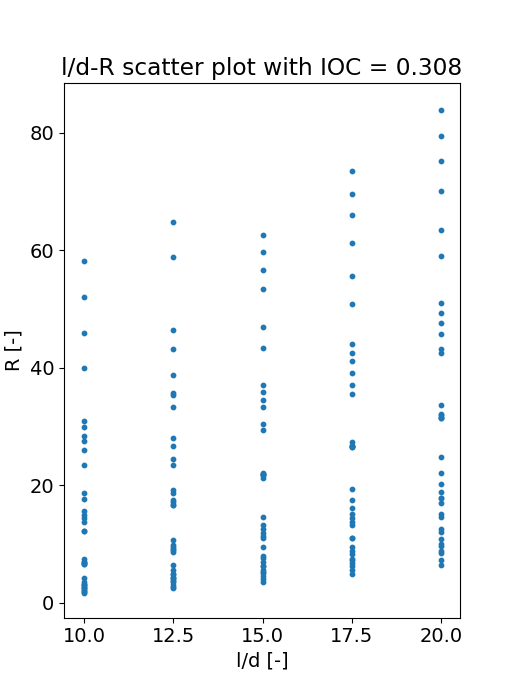
\includegraphics[width=.99\linewidth]{l2d_R}
  \caption{$l/d-R$}
\end{subfigure}
~
\begin{subfigure}[b]{.32\textwidth}
  \centering
  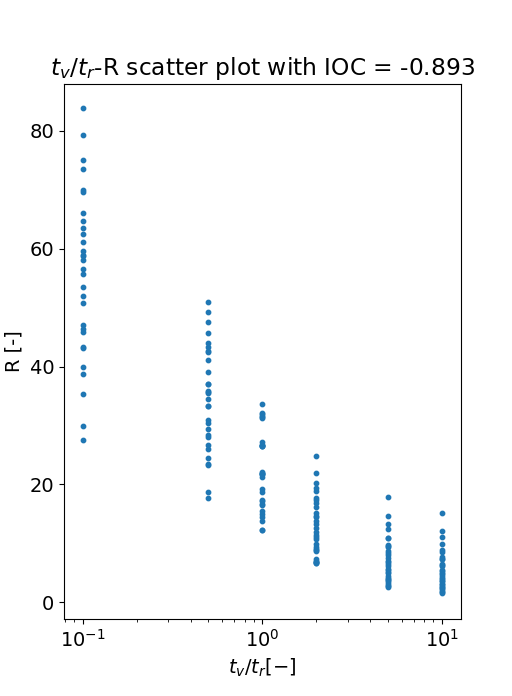
\includegraphics[width=.99\linewidth]{gamma_R}
  \caption{$t_v/t_r-R$}
\end{subfigure}

\caption{Geometric parameters-response factor scatter plot}
\label{fig:geom-R_scatter}
\end{figure}


\subsection{Influence of modal parameters}
\label{subsec:influence of modal parameters}
The influence of geometric parameters on the response factor is actually not direct. Whatever the change in geometry, it will firstly reflected in the modal properties, and then the dynamic performance. The relation between geometry and modal properties has been explored in section \ref{sec:modal analysis}. The next step would be to analyze how the modal parameters influences the dynamic behavior. As the modal parameters are always related to a certain mode, a clear relation only exists in the modal properties and the modal response resulted from them. Since the first mode makes the overwhelmingly dominant contribution to total response, the findings related to the first mode can be applied to the overall behaviour to a great extent.

Modal mass, natural frequency and mode shape are the three modal parameters that take part in the calculation and influence the response factor. Figure \ref{fig:m1,f1_R1_contour} shows the $m_1,f_1-R_1$ contour of different spans. "Coincidentally", the contour lines from different spans are in alignment with each other. This is actually no coincidence, no matter how different the geometry of two floors is, as long as they have the same modal properties, they are identical in modal space and have the same response. The small deviations among different spans may lie in the interpolation when making the contours and the similar but not identical mode shapes. 

It can be found that a higher natural frequency and a greater modal mass will both contribute to a lower response factor, but to a different degree depending on the initial situation. The gradient of the contour lines implies that the frequency has a greater impact when the modal mass is already high, or when the frequency is still low. The modal mass plays a greater role when the floor already shows a high frequency or a low modal mass. This finding indicates that if a floor has a very low modal mass or a very high natural frequency, the most efficient way to improve the dynamic performance is to increase the modal mass, instead of trying to further raise its natural frequency, and vice versa. This may further imply that, for a floor with a short span, which is usually accompanied with a low modal mass, improvements should be taken to increase the modal mass. A thinkable way is to add mass where  necessary and efficient. Whereas for a large span floor, which is likely to already have a high modal mass, measures to increase the natural frequency will be preferred. Probably removing material from where redundant is better than adding mass. The high frequency of the vaulted floor is just achieved by removing redundant material. 

\begin{figure}[H]
\centering
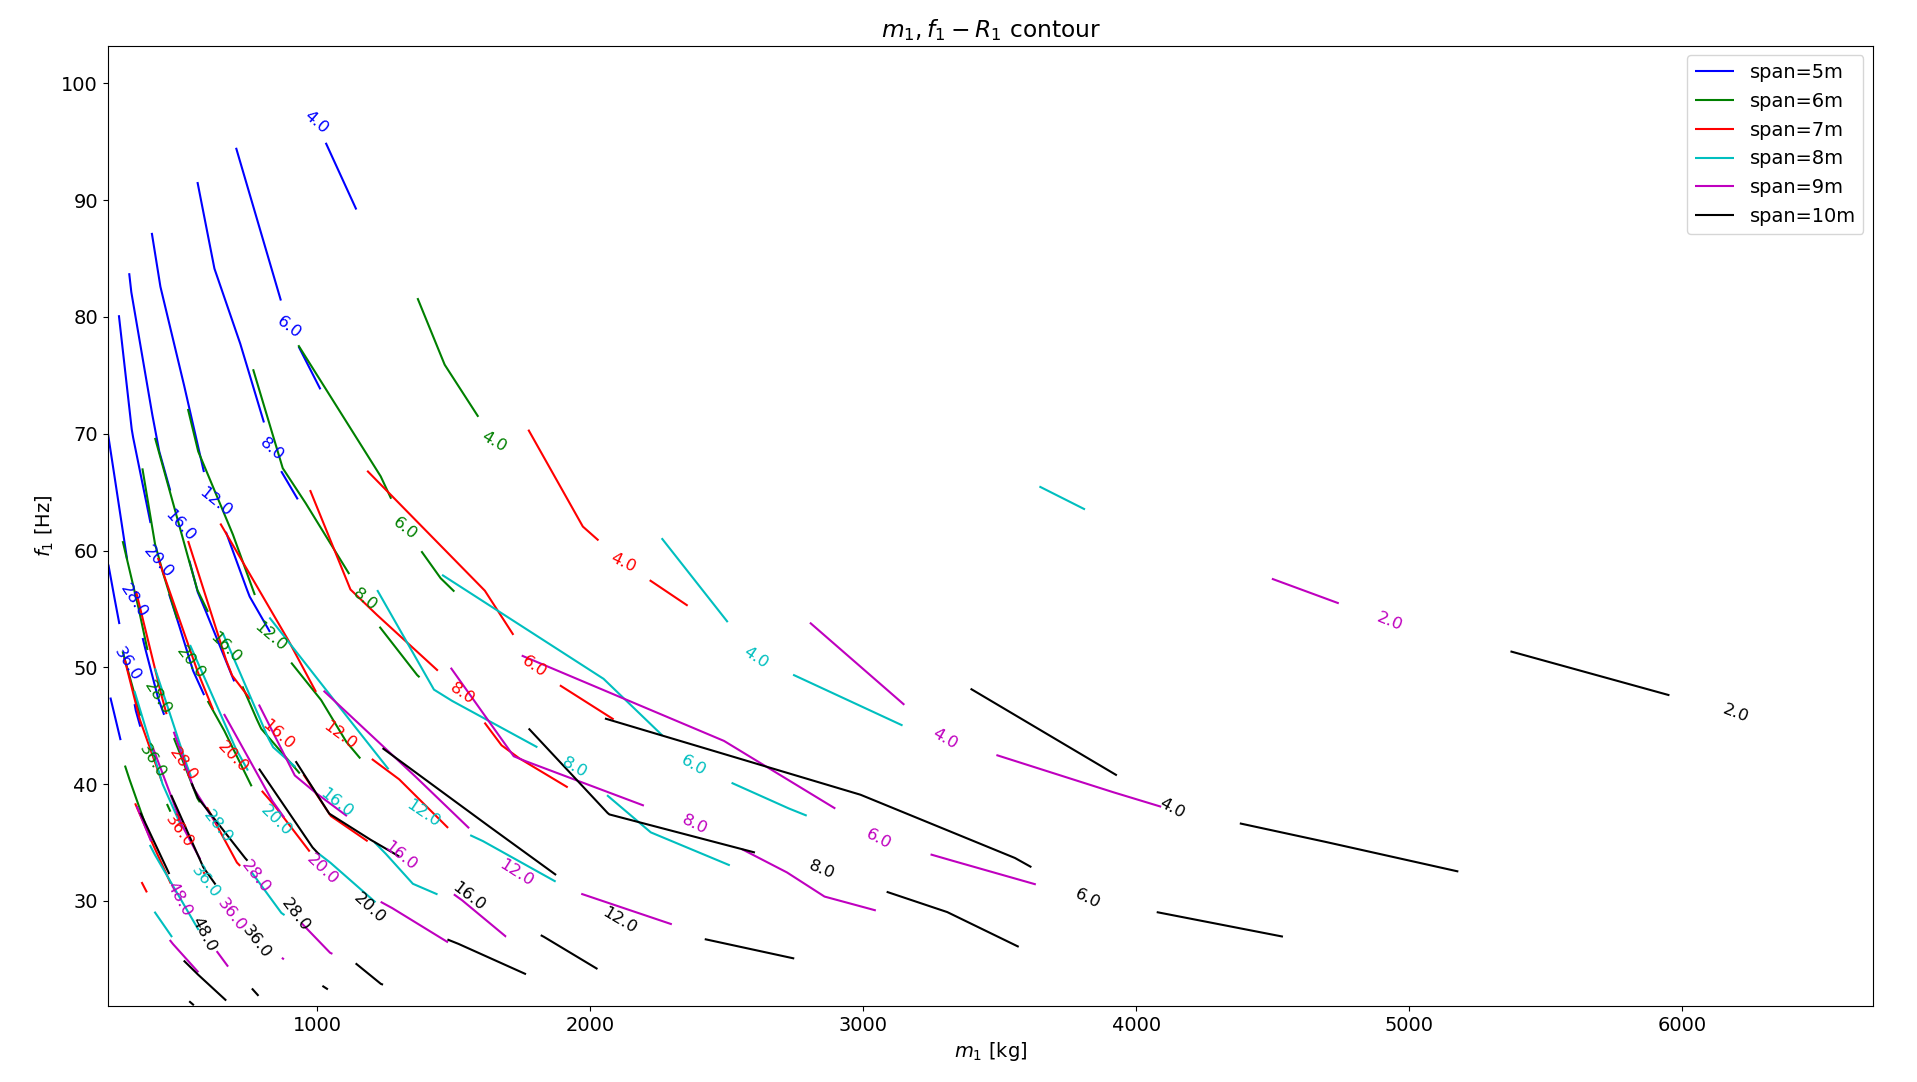
\includegraphics[width=1\textwidth]{images/m1,f1_R1}
\caption{$m_1,f_1-R_1$ contour plot}
\label{fig:m1,f1_R1_contour}
\end{figure}

As stated above, figure \ref{fig:m1,f1_R1_contour} is independent from the concrete geometry, this property may endow it a new utility - "table look-up". As long as $m_1$ and $f_1$ are known, the response factor can be directly read off or interpolated from this plot. The solution of response time history and post-processing of the data can be skipped, thus a quite amount of time can be saved. This can be practical for a quick check of the response after the modal analysis, it can also serve as the "objective function" to minimize for an optimization process. Compared with solely $m_1$ or $f_1$ as the objective function, $R_1$ is a more proper quantity that is directly associated with the actual performance. 

Figure \ref{fig:m1,f1_R1_contour} and figure \ref{fig:geom-R_contour} both describe the dynamic characteristics of the series of floors, but in a different way. The former is more for academic use, as the modal analysis has to be carried out as the first step. The independence from the concrete geometry makes it universal, it does not, however, provide any clue how to change $m_1$ and $f_1$ in an expected direction in the real world. Figure \ref{fig:geom-R_contour} is a rather engineer plot, which tells the engineer how to change the geometric parameters to achieve an acceptable performance, but it limits itself to a very specific geometry.

The influence of $m_1$ and $f_1$ on $R_1$ can also be depicted by input/output correlation plot, as shown in figure \ref{fig:m1,f1_R1_scatter}. The influence of the modal mass is enormous, very high responses are only possible when the modal masses are very low. The impact of the natural frequency is also considerable, the response factor tends to decrease when the natural frequency raises.

\begin{figure}[H]
\begin{subfigure}[b]{.49\textwidth}
  \centering
  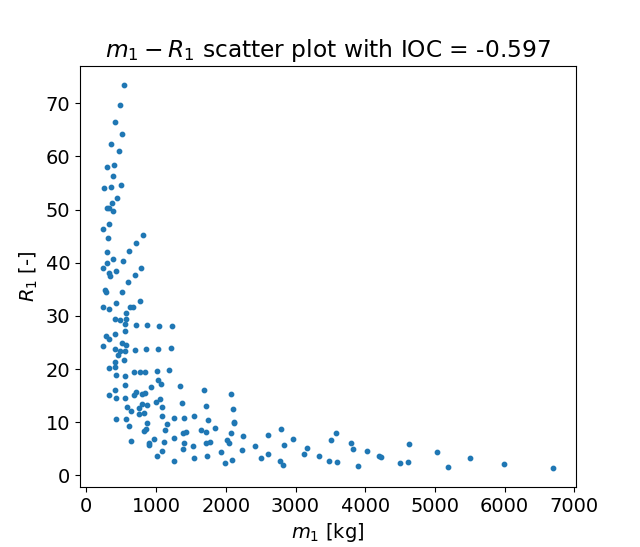
\includegraphics[width=.99\linewidth]{m1_R1}
  \caption{$m_1-R_1$}
\end{subfigure}
~
\begin{subfigure}[b]{.49\textwidth}
  \centering
  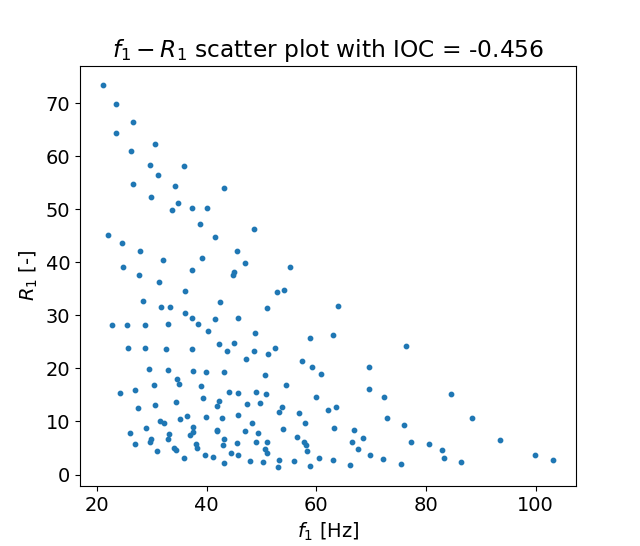
\includegraphics[width=.99\linewidth]{f1_R1}
  \caption{$f_1-R_1$}
\end{subfigure}

\caption{Modal parameter- modal response factor scatter plot}
\label{fig:m1,f1_R1_scatter}
\end{figure}

From the previous analysis, it can be concluded that $t_v/t_r, m_1, f_1$ are the three most important parameters that influence the response factor $R_1$. These parameters are not independent, it will be meaningful to see their correlation in one plot. Figure \ref{fig:norm_m1_f1_R1} illustrates the normalized $m_1,f_1,R_1$ (normalized by $t_v/t_r=0.1$) in relation to $t_v/t_r$. It shows a very interesting "mirrored" relation between normalized modal mass and normalized response factor while the normalized frequency keeps almost constant around 1. The "mirrored" relation in log scale indicates an inverse proportional relationship in normal scale, which is exactly the relation suggested by SCI P354 expressed in equation \ref{eqn:SCI} and by the calculation of participation factor $\Gamma_n$ expressed in equation \ref{eqn:Gamma}. This mirror is even rigorous in sequence in terms of specific $l$ and $l/d$. The mirror, however, is not very rigorous in values, for example, the normalized $m_1,f_1,R_1$ written in tuple ($m_{1,n},f_{1,n},R_{1,n}$)=(20.23,1.42,0.029) for $l=5m, l/d=10, t_v/t_r=10$, the product of $m_{1,n}\times R_{1,n}=20.23\times 0.029=0.59$ is not even close to 1, that lies in the normalized frequency that deviates already considerably from 1 (the influence of frequency will be discussed later). This plot also shows the great improvements that can be achieved by changing the $t_v/t_r$ ratio, the response could drop to 3\%-25\% of the response with $t_v/t_r=0.1$. Such great improvements are directly related to the huge increase in modal mass.
\begin{figure}[H]
\centering
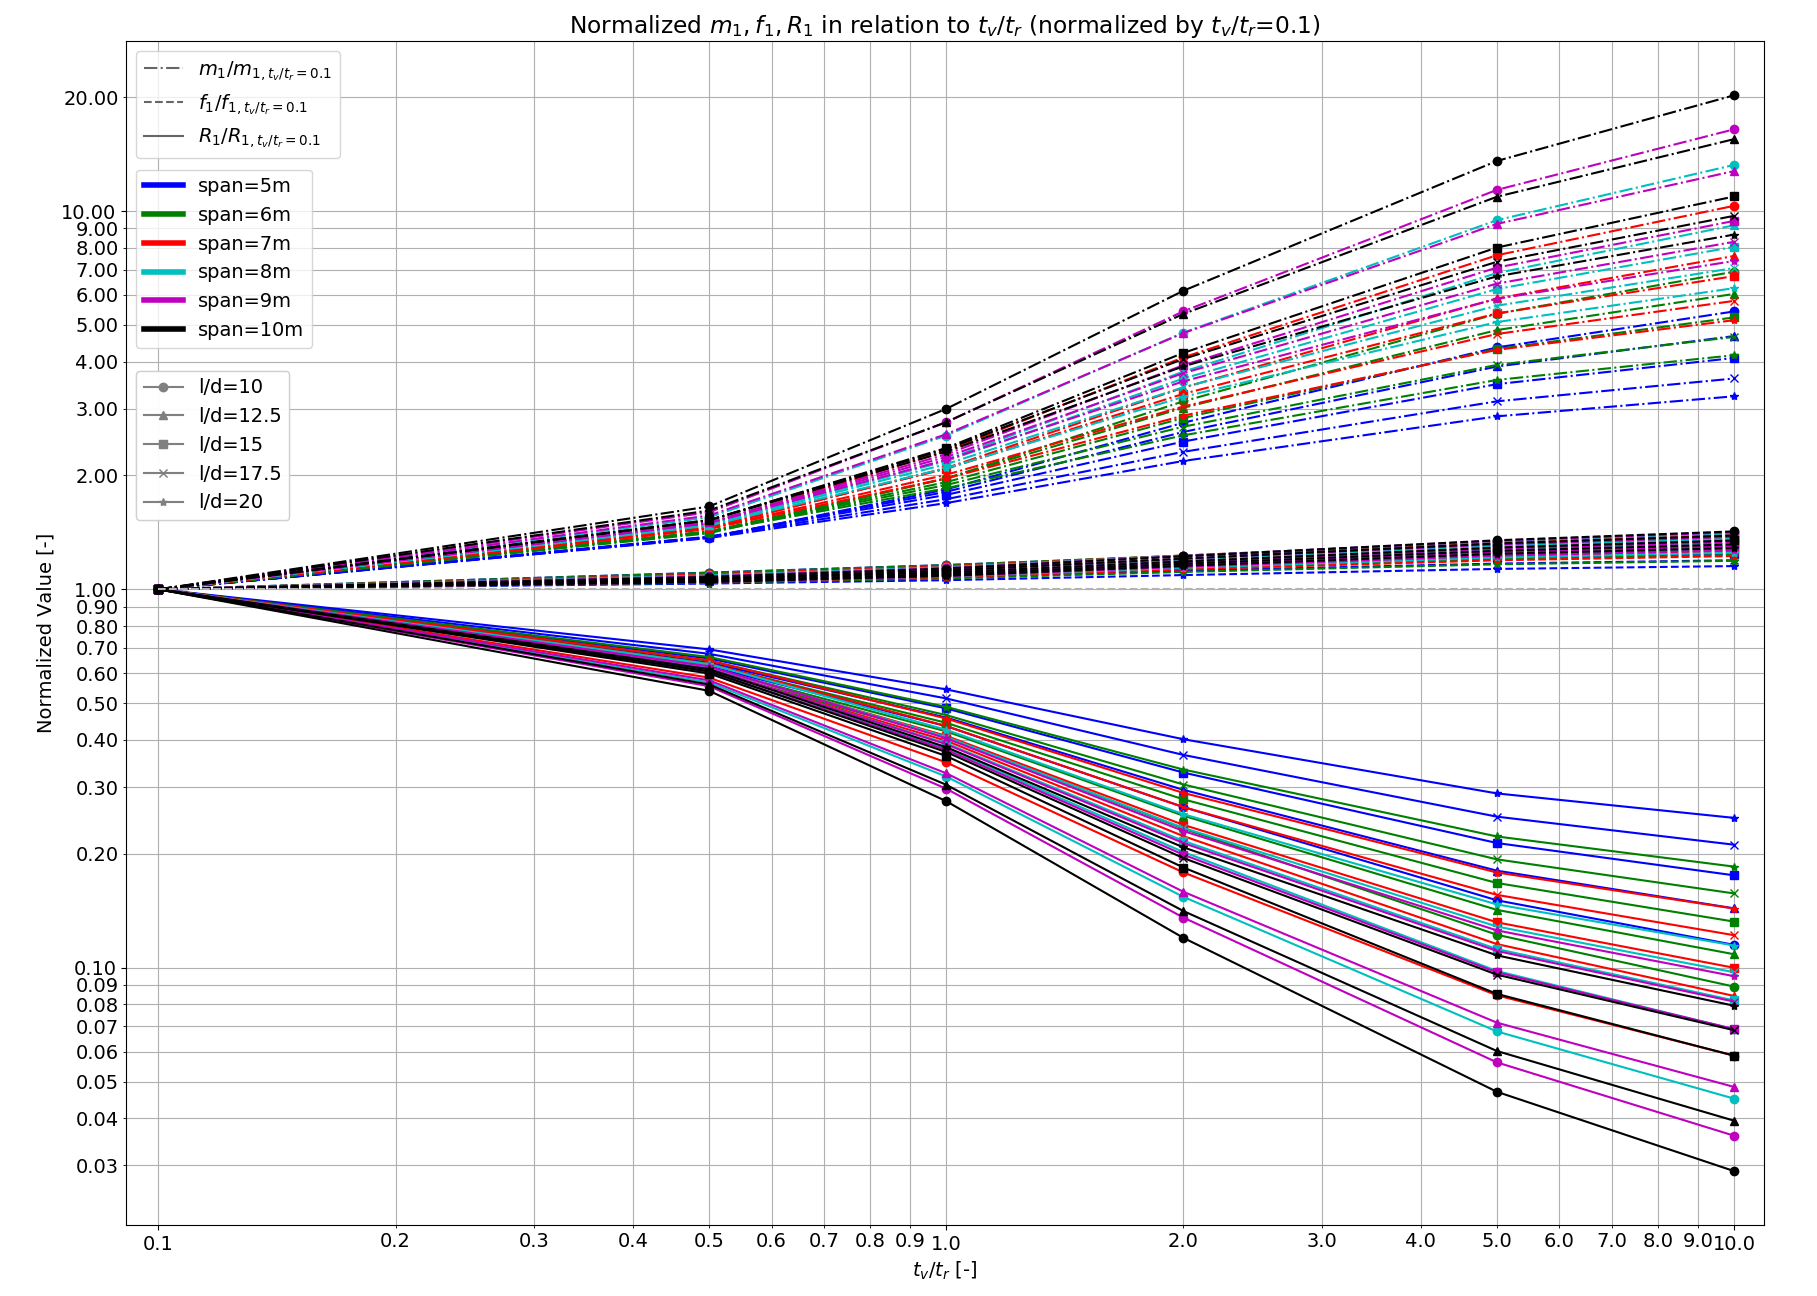
\includegraphics[width=1\textwidth]{images/norm_m1_f1_R1}
\caption{Normalized $m_1,f_1,R_1$ in relation to $t_v/t_r$}
\label{fig:norm_m1_f1_R1}
\end{figure}

The mathematical relation between natural frequency and response factor is less direct. To ward off the influence of the modal mass, ($m_1,f_1,R_1$) tuples with constant $m_1$ should be selected. One can see from figure \ref{fig:m1,f1_R1_scatter} that there are relative concentrated points around $m_1=850$ kg. 18 points with $m_1=[1\pm10\%]\times850$ kg are chosen, and normalized by point 0 with ($m_1,f_1,R_1$)=(813.0,22.0,45.1). Figure \ref{fig:norm_m1_f1_R1_const_m1} shows the results. It depicts a roughly mirrored figure, but the normalized $f_1$ values seem to be not high enough in position. When the exponent of $f_1$ is raised to 1.5, the figure turns out to present a well shaped mirrored figure, as shown in figure \ref{fig:norm_m1_f1_1_5_R1_const_m1}. It means that the response factor is in inverse proportion to $f_1^{1.5}$ when the $m_1$ keeps constant. The over inverse proportional relation is not without reason. Firstly, the natural frequency influences the response factor through the frequency weighting function (see figure \ref{fig:Wb}) $W_b=16/f_1$ when $f_1>16$ Hz, which applies to all floors. Secondly, the natural frequency also intervenes in the solution of response time history expressed in equation \ref{eqn:motion_q}, a raise in $\omega_n$ will lead to a drop in $q_n(t)$, and thus in response. 
\begin{figure}[H]
\centering
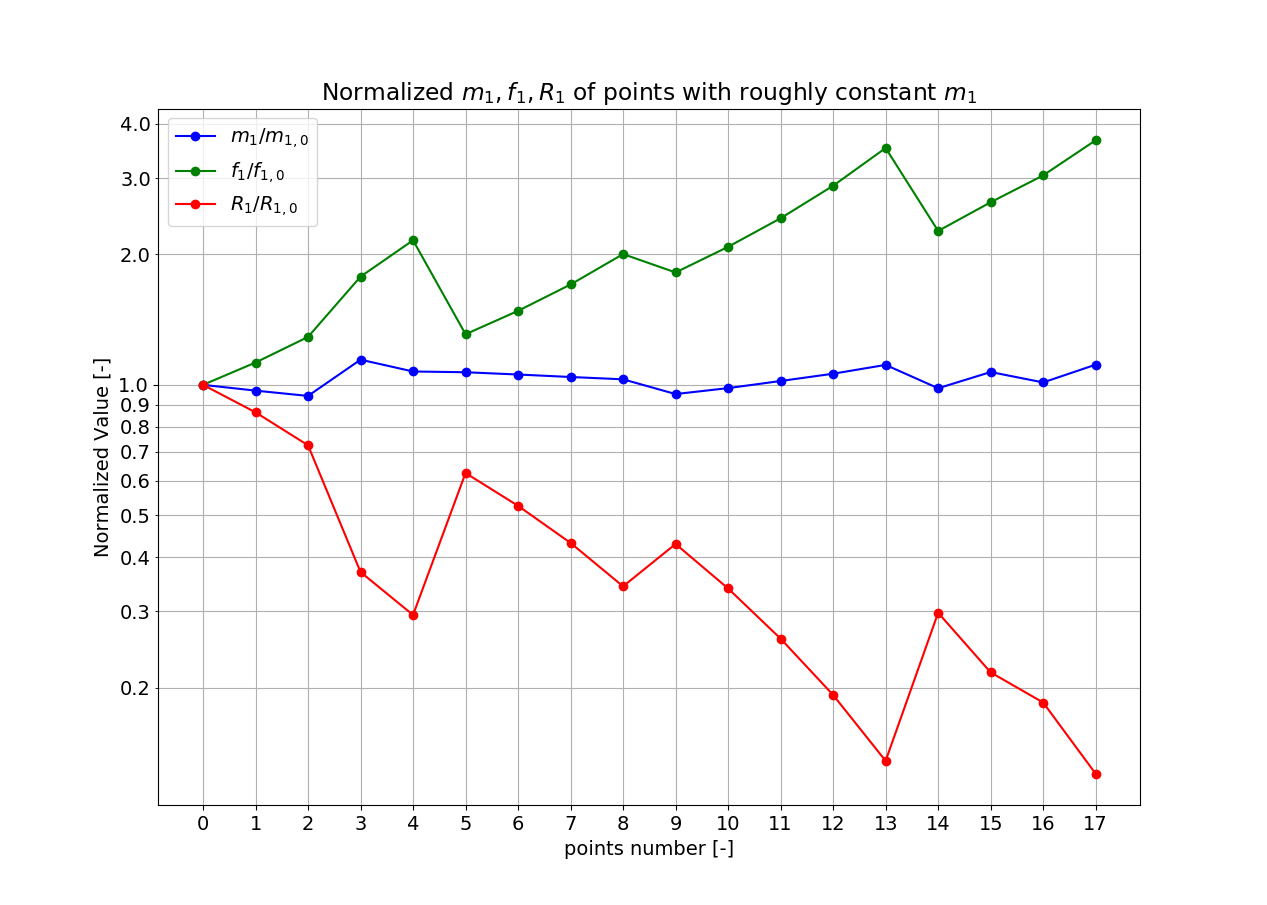
\includegraphics[width=.8\textwidth]{images/norm_m1_f1_R1_const_m1.png}
\caption{Normalized $m_1,f_1,R_1$ of points with roughly constant $m_1$}
\label{fig:norm_m1_f1_R1_const_m1}
\end{figure}

\begin{figure}[H]
\centering
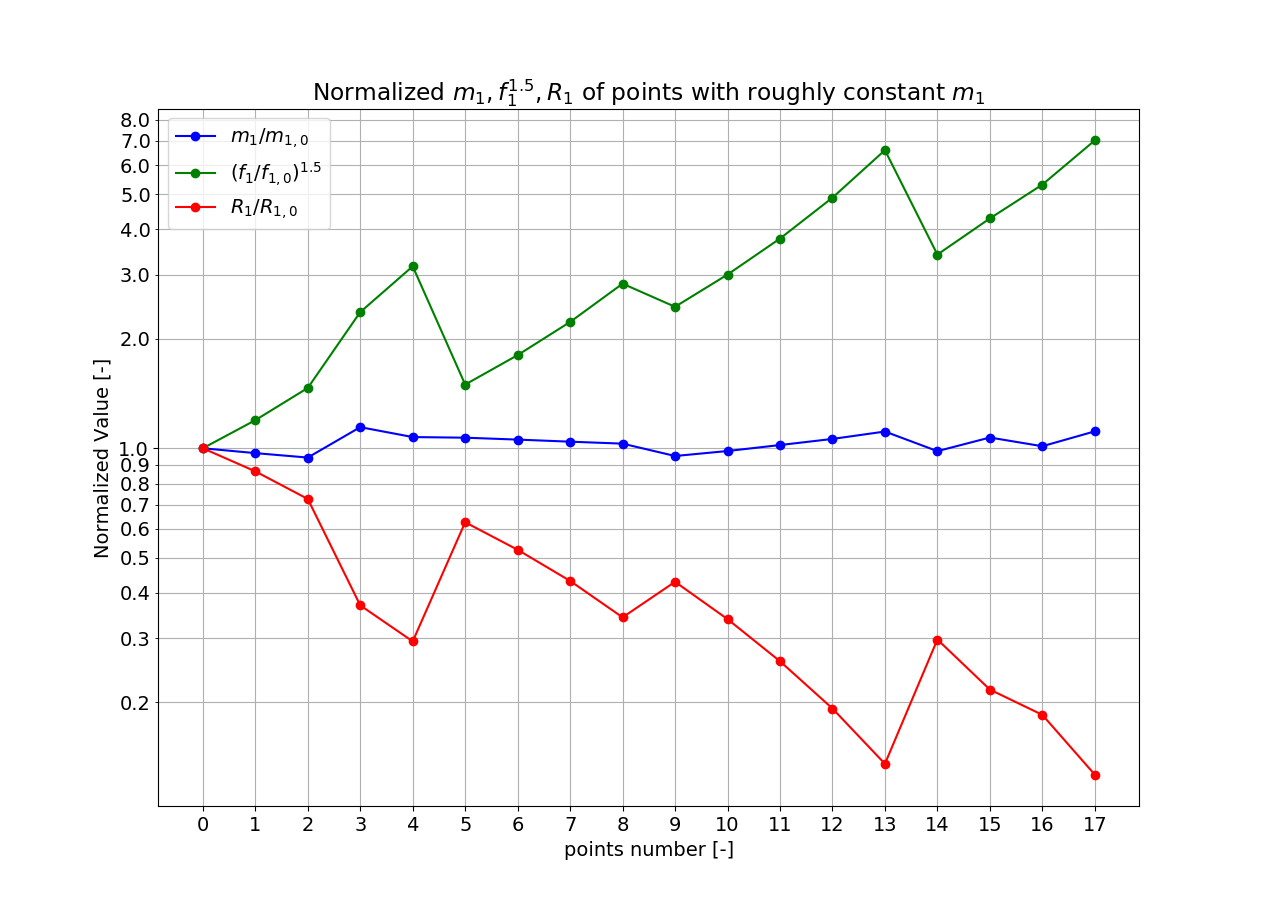
\includegraphics[width=.8\textwidth]{images/norm_m1_f1_1_5_R1_const_m1.png}
\caption{Normalized $m_1,f_1^{1.5},R_1$ of points with roughly constant $m_1$}
\label{fig:norm_m1_f1_1_5_R1_const_m1}
\end{figure}

Combining the effect of modal mass and natural frequency, the response factor can be expressed as:
\begin{equation}
    R_1\sim \frac{1}{m_1f_1^{1.5}}
\label{eqn:R1}
\end{equation}
When the tuple ($m_{1,n},f_{1,n},R_{1,n}$)=(20.23,1.42,0.029) is used to calibrate this formula:
\begin{equation}
    \frac{1}{m_{1,n}f_{1,n}^{1.5}}=\frac{1}{20.23\times1.42^{1.5}}=0.029\approx R_{1,n}
\label{eqn:R1_n}
\end{equation}
they match very well.

Note that equation \ref{eqn:R1} only represents a proportional relation, not a concrete formula, it applies to \ref{eqn:R1_n} as there normalized values are used. The equivalent expression would be:
\begin{equation}
    R_1= \frac{C}{m_1f_1^{1.5}}
\label{eqn:R1(m1_f1)}
\end{equation}
where $C$ is a constant that can be obtained by calculating the mean of all data points. After evaluation, the constant $C=3778622$. 

Figure \ref{fig:m1,f1_R1_pred} shows the true and predicted data points in modal space. The precision of prediction is measured by the MSE (mean square error) index
\begin{equation}
    MSE=\frac{1}{n}\sum_{i=1}^n(\hat{y}_i-y_i)^2
\end{equation}
\noindent
The true and predicted data points are almost superposed, the $MSE$ is as low as 0.264\%. Equation \ref{eqn:R1(m1_f1)} unveils the quantitative relation between modal response factor and modal parameters, which may make further response time history analysis redundant. It needs to be pointed out that this equation is only valid for floors with natural frequency $f_1>16$ Hz, otherwise the frequency weighting function $W_b$ will have other forms, so will this equation. That is probably is reason why this formula differs from equation \ref{eqn:SCI} greatly in the exponent of $f_1$.

\begin{figure}[H]
\begin{subfigure}[b]{.49\textwidth}
  \centering
  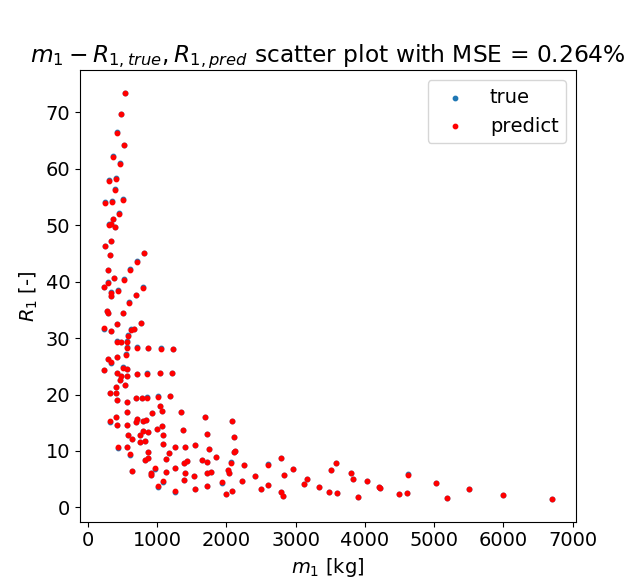
\includegraphics[width=.99\linewidth]{m1_R1_pred}
  \caption{$m_1-R_{1,\text{true}},R_{1,\text{pred}}$}
\end{subfigure}
~
\begin{subfigure}[b]{.49\textwidth}
  \centering
  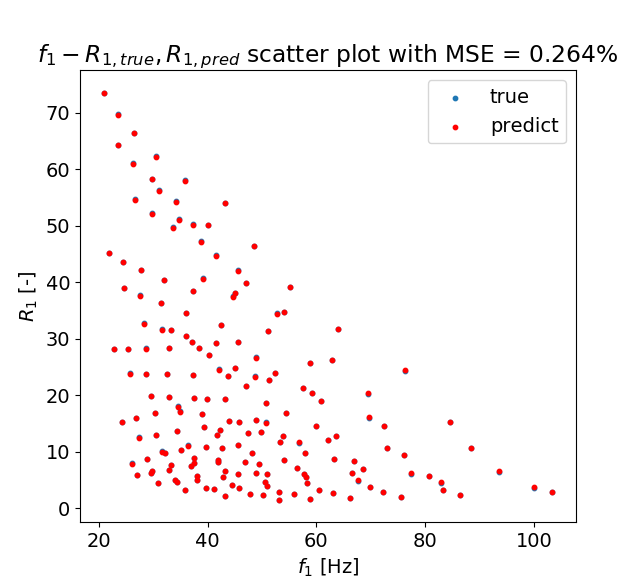
\includegraphics[width=.99\linewidth]{f1_R1_pred}
  \caption{$f_1-R_{1,\text{true}},R_{1,\text{pred}}$}
\end{subfigure}

\caption{True and predicted modal response factor in modal space}
\label{fig:m1,f1_R1_pred}
\end{figure}

The natural frequency seems to have less impact than the modal mass according to figure \ref{fig:m1,f1_R1_scatter}. This misconception stems from the narrower value range of natural frequency. The natural frequency ranges from 20 Hz to 100 Hz (5 times), while modal mass from 230 kg to 6700 kg (29 times), so the effect of modal mass seems much more dramatic. Nonetheless, these ranges may also indicate the relative difficulty in changing the two parameters.